\documentclass[10pt, a4j, dvipdfmx]{jarticle}
\usepackage{titlesec}
\usepackage[dvipdfmx]{graphicx}
\usepackage[dvipdfmx]{color}
\usepackage{float}
\usepackage{wrapfig}
\usepackage{subfigure}
\usepackage{caption}
\usepackage{multirow}

\graphicspath{{../images/}}

\makeatletter
\newcommand{\figcaption}[1]{\def\@captype{figure}\caption{#1}}
\newcommand{\tblcaption}[1]{\def\@captype{table}\caption{#1}}
\makeatother

\title{トランジスタ増幅}
\author{4年 電子システム工学科 40番  山地 駿徹}


\begin{document}
    \section{実験方法}
    \subsection{トランジスタの静特性}

    \subsubsection{入力特性の測定方法}
    エミッタ接地回路で,$V_{CE}$を一定に保ち,$V_{BE}$を変化させたときの$I_B$の変化を測定する.
    \begin{figure}[H]
        \begin{minipage}{0.5\hsize}
            \centering
            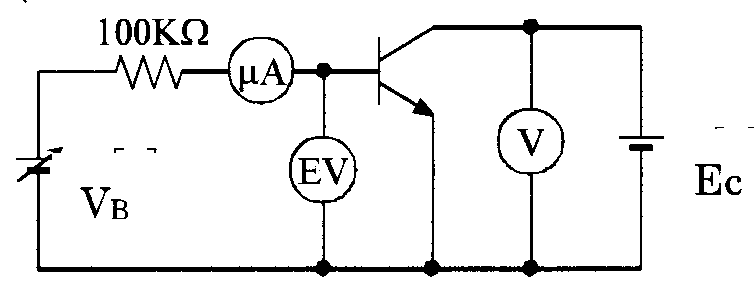
\includegraphics[width=50mm]{fig-1.png}
            \caption{入力特性測定回路}
            \label{fig:1}
        \end{minipage}
        \begin{minipage}{0.5\hsize}
            \centering
            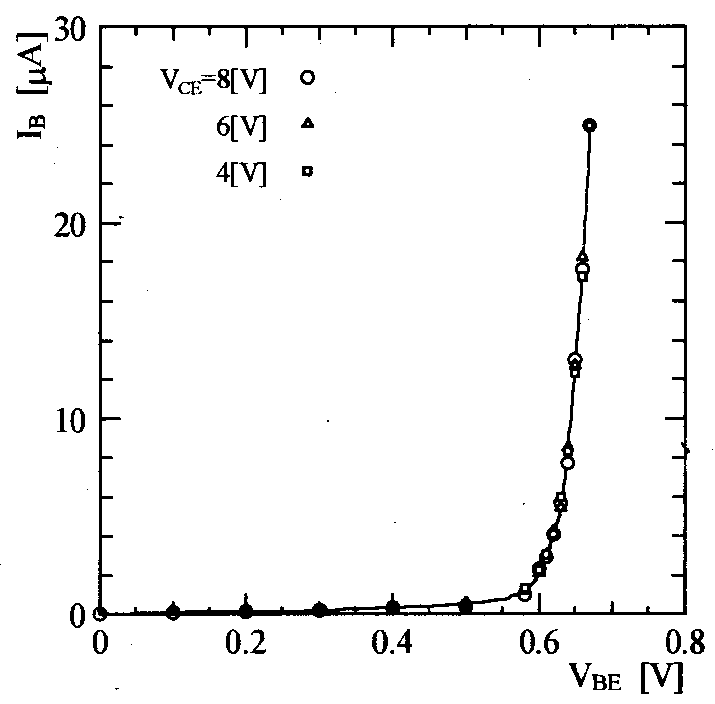
\includegraphics[height=45mm]{fig-2.png}
            \caption{入力特性}
            \label{fig:2}
        \end{minipage}
    \end{figure}

    \subsubsection{出力特性の測定方法}
    エミッタ接地回路で,$I_B$を一定に保ち,$V_{CE}$を変化させたときの$I_C$の変化を測定する.
    \begin{figure}[H]
        \begin{minipage}{0.5\hsize}
            \centering
            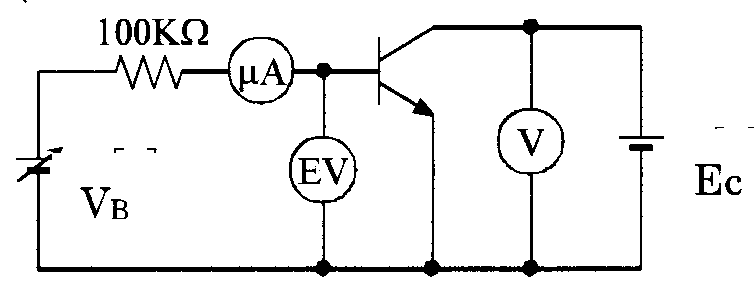
\includegraphics[width=50mm]{fig-1.png}
            \caption{出力特性測定回路}
            \label{fig:3}
        \end{minipage}
        \begin{minipage}{0.5\hsize}
            \centering
            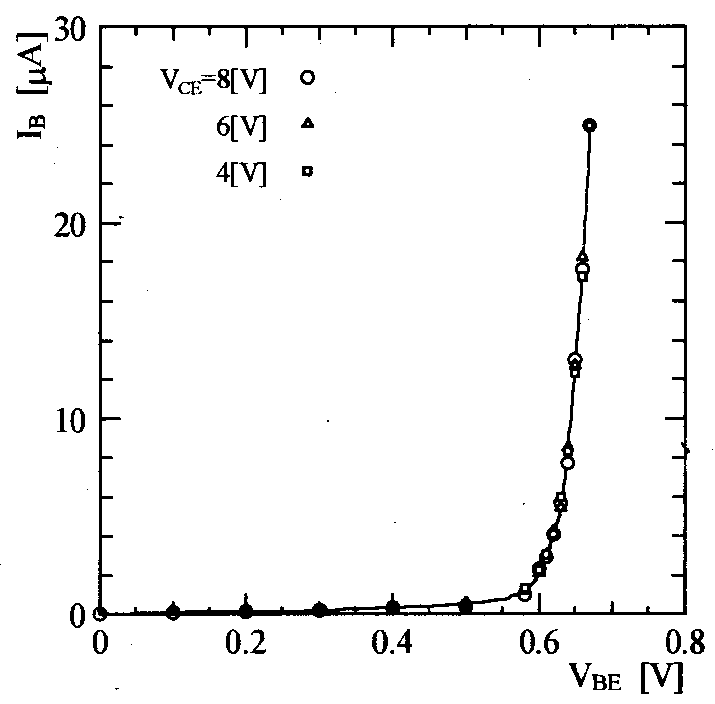
\includegraphics[height=45mm]{fig-2.png}
            \caption{出力特性}
            \label{fig:4}
        \end{minipage}
    \end{figure}
    \subsubsection{吟味事項}
    \begin{enumerate}
        \item 電圧計,電流計の等級と内部抵抗を調べる.\\電圧計,電流計の接続方法により,計器の内部抵抗による測定誤差について考察する.\\その時の補正方法を考察する.
        \item $V_{CE} = 4[V]$,$I_B = 20[\mu A]$のときの$h$定数を,測定した特性図より求める.
    \end{enumerate}

    \newpage
    \subsection{トランジスタ増幅}

    \subsubsection{電流増幅特性の測定方法}
    エミッタ接地回路で$R_C = 1[k\Omega]$を接続し$E_C = 8[V]$一定として,$I_B$を変化させたときの$I_C$の変化を測定する.
    \small (注. 電流計の内部抵抗が負荷抵抗に加算されないように$E_C$を調整する)
    \normalsize
    \begin{figure}[H]
        \begin{minipage}{0.5\hsize}
            \centering
            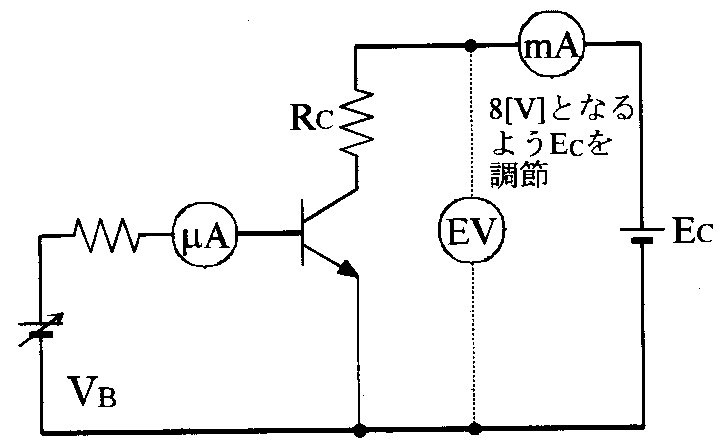
\includegraphics[width=50mm]{fig-5.png}
            \caption{電流増幅特性測定回路}
            \label{fig:5}
        \end{minipage}
        \begin{minipage}{0.5\hsize}
            \centering
            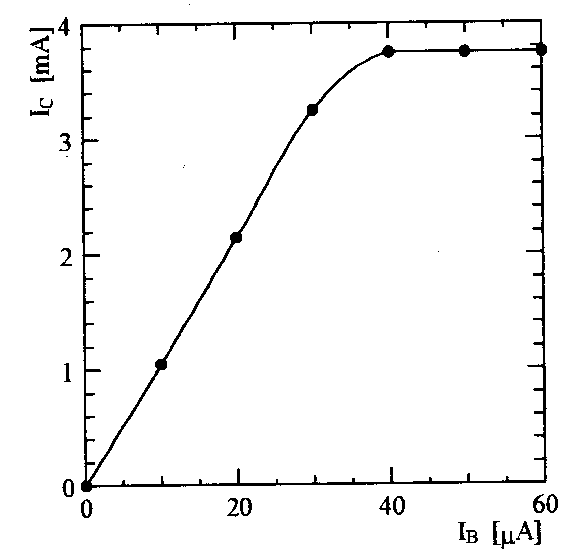
\includegraphics[height=45mm]{fig-6.png}
            \caption{電流増幅特性}
            \label{fig:6}
        \end{minipage}
    \end{figure}

    \subsubsection{電圧増幅特性の測定方法}
    エミッタ接地回路で$R_C = 1[k\Omega]$を接続し$E_C = 8[V]$一定として,$V_{BE}$を変化させたときの$V_{CE}$の変化を測定する.
    \begin{figure}[H]
        \begin{minipage}{0.5\hsize}
            \centering
            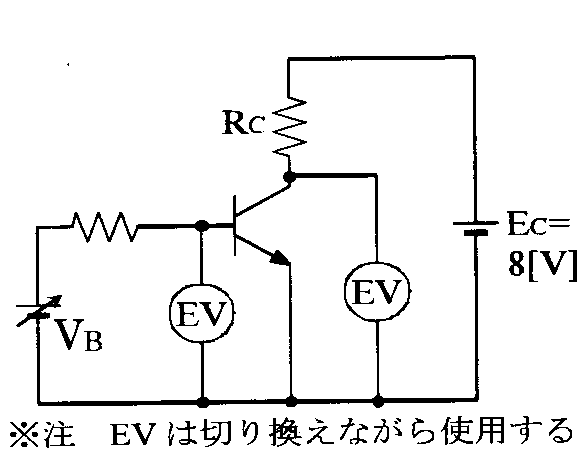
\includegraphics[width=50mm]{fig-7.png}
            \caption{電圧増幅特性測定回路}
            \label{fig:7}
        \end{minipage}
        \begin{minipage}{0.5\hsize}
            \centering
            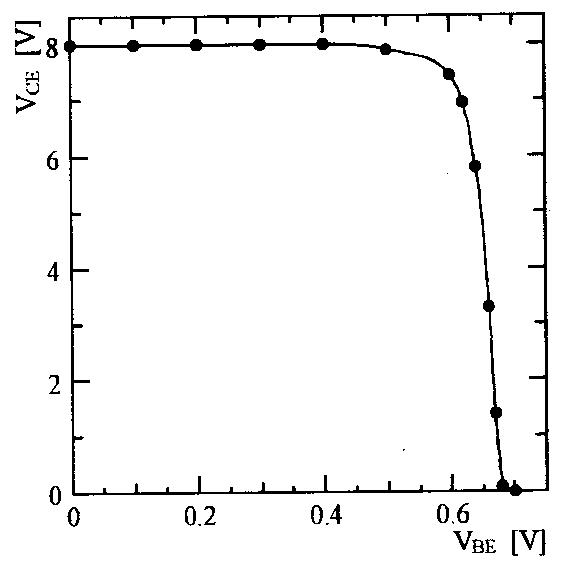
\includegraphics[height=45mm]{fig-8.png}
            \caption{電圧増幅特性}
            \label{fig:8}
        \end{minipage}
    \end{figure}

    以上の測定はトランジスタ増幅回路の交流不可線上の特性を測定することと等価である.\\
    まず,動作点$Q$を電流増幅特性の直線部分より決定する.次に,この動作点に対応する電圧増幅特性での動作点を記入する.

    \subsubsection{吟味事項}
    \begin{enumerate}
        \item 電流増幅特性より,$h_{FE}$を求める.
        \item 電圧増幅特性より電圧増幅度を求める.
    \end{enumerate}

    \newpage
    \subsubsection{直流バイアス回路定数の選定及びバイアス電圧測定}
    \begin{wrapfigure}{r}{70mm}
        \vspace*{-\intextsep}
        \begin{center}
            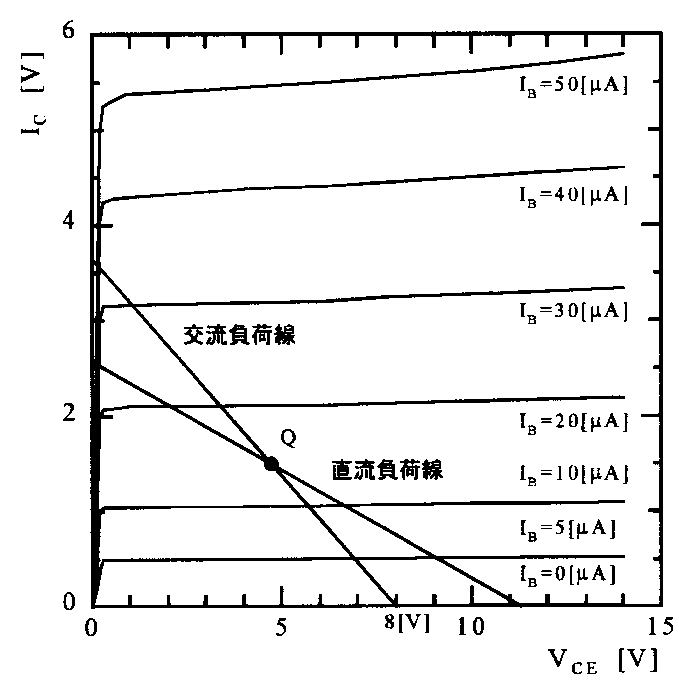
\includegraphics[height=50mm]{fig-9.png}
            \label{fig:9}
            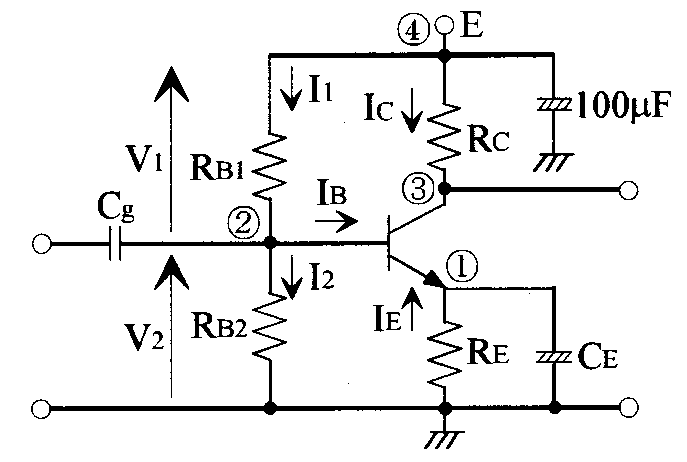
\includegraphics[height=40mm]{fig-10.png}
            \caption{出力特性測定回路}
            \label{fig:10}
        \end{center}
    \end{wrapfigure}
    先の実験で測定した出力特性に$8[V]$,$R_C$の交流負荷線を引き,動作点を記入する.\\ 
    \begin{equation}
        E_C = R_C I_C + V_{CE}
    \end{equation}
    また,動作点を通る傾き$1/(R_C + R_E)$の直流負荷線を引き,電源電圧を決定する.\\
    ここでは$R_C = R_E = 1k\Omega$とする.

    以下の下線部を埋めて実験を行う.\\
    Trの名称\hspace{25mm}\underline{\hspace{30mm}}\\
    交流負荷線 $R_C = $    \underline{\hspace{20mm}}$\Omega$\\
    直流負荷線 $R_C + R_E = $  \underline{\hspace{20mm}}$\Omega$\\
               $R_E = $     \underline{\hspace{20mm}}$\Omega$\\
    \\
    電源電圧 $E = $ \underline{\hspace{20mm}}$V$\\
    設定した動作点Qにおける\\
    ベース電流 $I_{BQ} = $ \underline{\hspace{20mm}}$\mu A$\\
    コレクタ電流 $I_{CQ} = $ \underline{\hspace{20mm}}$mA$\\
    電流増幅率 \underline{\hspace{20mm}}\\
    ベース-エミッタ間電圧 $V_{BEQ} = $ \underline{\hspace{20mm}}$V$\\
    コレクタ-エミッタ間電圧 $V_{CEQ} = $ \underline{\hspace{20mm}}$V$\\
    \\
    静特性から,図\ref{fig:10}における各点の電位は,\\
    \hspace{7mm}\textcircled{\scriptsize 1} \underline{\hspace{20mm}}$V$\hspace{7mm}\textcircled{\scriptsize 2} \underline{\hspace{20mm}}$V$\hspace{7mm}\textcircled{\scriptsize 3} \underline{\hspace{20mm}}$V$\\
    また,$I_2 = V_2 / R_{B2}$,$I_1 = (E - V_2)$,$I_1 = I_2 + I_{BQ}$の関係が成り立つ.\\
    $I_{BQ}$,$V_1$,$V_2$,$E$は既知である.また,係数$k$を導入し,$I_2 = k I_{BQ}$と表す.これらを用いて$I_1$,$I_2$,$R_{B1}$,$R_{B2}$を式で表すと\\
    \hspace{7mm}$I_1 = $ \underline{\hspace{20mm}}\hspace{7mm}$I_2 = $ \underline{\hspace{20mm}}\hspace{7mm}$R_{B1} = $ \underline{\hspace{20mm}}$R_{B2} = $ \underline{\hspace{20mm}}\\
    となる.$k$の値を変えていくつかの場合について$R_{B1}$,$R_{B2}$の値を求めよ.一番右端の欄には,実験回路に選んだ値を記せ.
    \begin{table}[H]
        \begin{tabular}{||c||c|c|c|c|c|c||c||}
        \hline\hline
        $k$      & $1$           & $5$           & $10$          &               &               &               &               \\ \hline\hline
        $R_{B1}$ & \hspace{15mm} & \hspace{15mm} & \hspace{15mm} & \hspace{15mm} & \hspace{15mm} & \hspace{15mm} & \hspace{15mm} \\ \hline
        $R_{B2}$ &               &               &               &               &               &               &               \\ \hline\hline
        \end{tabular}
    \end{table}
    \newpage
    増幅しようとする周波数範囲は,\hspace{7mm}\underline{\hspace{20mm}}$Hz$〜\hspace{7mm}\underline{\hspace{20mm}}$Hz$\\
    この下限周波数より,$C_g$,$C_E$を決定すると,$C_g = $\underline{\hspace{20mm}}$\mu F$\hspace{7mm} \underline{\hspace{20mm}}$\mu F$\\
    各点の電位及び電圧
    \begin{table}[H]
        \begin{tabular}{||c||c|c|c||c||c|c|c||}
        \hline\hline
        点                           & 設計値           & 実測値           & 誤差            & 点                                                           & 設計値           & 実測値           & 誤差            \\ \hline\hline
        \textcircled{\scriptsize 1} & \hspace{15mm} & \hspace{15mm} & \hspace{15mm} & $\textcircled{\scriptsize 3} - \textcircled{\scriptsize 1}$ & \hspace{15mm} & \hspace{15mm} & \hspace{15mm} \\ \hline
        \textcircled{\scriptsize 2} &               &               &               & $\textcircled{\scriptsize 2} - \textcircled{\scriptsize 1}$ &               &               &               \\ \hline
        \textcircled{\scriptsize 3} &               &               &               & $\textcircled{\scriptsize 4} - \textcircled{\scriptsize 2}$ &               &               &               \\ \hline
        \textcircled{\scriptsize 4} &               &               &               & $\textcircled{\scriptsize 4} - \textcircled{\scriptsize 3}$ &               &               &               \\ \hline\hline
        \end{tabular}
    \end{table}

    \subsubsection*{補足:直流バイアス回路の設計}
    \begin{wrapfigure}{r}{30mm}
        \vspace*{-\intextsep}
        \begin{center}
            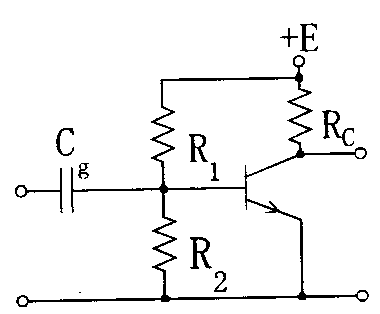
\includegraphics[width=30mm]{fig-11.png}
            \caption{}
            \label{fig:10}
        \end{center}
    \end{wrapfigure}
    トランジスタの静特性(出力特性)に交流負荷線$R_C$を引き,動作点$Q$を設定する.
    
    このとき,トランジスタに流れるベース電流$I_{BQ}$,コレクタ電流$I_{CQ}$,ベース-エミッタ間電圧$V_{BEQ}$,コレクタ-エミッタ間電圧$V_{CEQ}$をトランジスタの静特性より求める.

    求めた$I_{BEQ}$,$I_{CEQ}$が流れるように
    \begin{equation}
        V_2 = \{R_2 / (R_1 + R_2)\} E = V_{BEQ}
    \end{equation}
    から$R_1$,$R_2$の値を設定する.

    これで良いのであるが,トランジスタは温度によって特性が変化する.特性が変化すると設定した動作点qがずれてしまい増幅器の特性も安定しなくなる.\\
    \begin{wrapfigure}{r}{30mm}
        \vspace*{-\intextsep}
        \begin{center}
            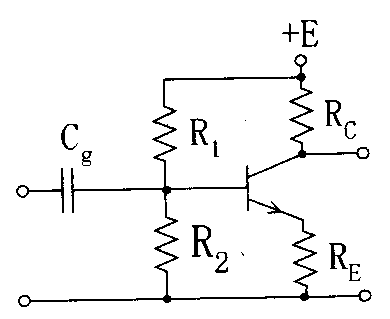
\includegraphics[width=30mm]{fig-12.png}
            \caption{}
            \label{fig:11}
        \end{center}.・
    \end{wrapfigure}.・
    そこで負帰還をかけて特性の変化による動作店の変動を.・抑制するため図\ref{fig:11}のように$R_E$を接続する.

    このとき,$R_C + R_E$は直流負荷線として図\ref{fig:9}のように静特性上に交流負荷線の動作点$Q$で交わる直線として引く.
    電源電圧$E$は$8V$から$R_E$による電圧降下分を加えた12Vに変わる.\\
    温度が交渉してベース電流が$I_{BQ}$よりも増加したとすると$R_E$による電圧降下は,
    \begin{equation}
        R_E(I_B + I_C) = R_E(I_{BQ} + I_{CQ} + \Delta I_B + \Delta I_C)
    \end{equation}\\
    となり,$R_E(\Delta I_B + \Delta I_C)$だけ$R_E$による電圧降下は大きくなる.\\
    $V_2$が一定であると仮定すると,
    \begin{equation}
        V_{BE} = V_2 - R_E(I_B + I_C) = V_2 - R_E(I_{BQ} + I_{CQ} + \Delta I_B + \Delta I_C)
    \end{equation}\\
    なので$I_B$が増加すると$V_{BE}$は小さくなる.$V_{BE}$が小さくなると$I_B$は減少する.
    このように$R_E$を接続することにより,ベース電流が増加(減少)しようとすると負帰還が働きベース電流の増加(減少)を押さえ,ベース電流を一定に保つ.

    次に,前述の解析では,$V_2$が一定であると仮定したわけであるが,$V_2$を一定にするためには,$R_2$にながれる電流$I_2$と$I_{BQ}$の比を大きくするとよい.
    $I_B$が増加するとその文だけ$I_2$は減少するが,比が大きいと$I_2$にとってその変化分はわずかな変化でしかなく,
    \begin{equation}
        V_2 = R_2 \cdot I_2 \approx 一定
    \end{equation}\\
    となる.

    今回の設計では,$I_ = k I_{BQ}$という定数$k$を導入する.
    $k$の値を大きくするほうが安定度は良いのであるだ,kを大きくしすぎると$R_1$と$R_2$の値が小さくなりすぎる.
    市販品の少抵抗は少なく,誤差も大きい.
    また,消費電力$R_2 \cdot I_2^2$が大きくなってよくない.
    消費電力が大きくなると発熱し,トランジスタの周囲温度を上げ,特性の変化をもたらす.\\
    \emph{ここでは,$R_1$と$R_2$の値は数$k\Omega$〜数$10k\Omega$程度になるように$k$を選ぶとよい.}

    \newpage
    \subsubsection{入出力特性の測定方法}
    設計製作した増幅回路に,低周波発振器より$f = 1kHz$の正弦波信号を入力する.
    この入力信号の入力電圧に対する出力電圧の変化を測定する.
    オシロスコープで入力波形と出力波形の変化も観測する.
    \begin{figure}[H]
        \begin{minipage}{0.5\hsize}
            \centering
            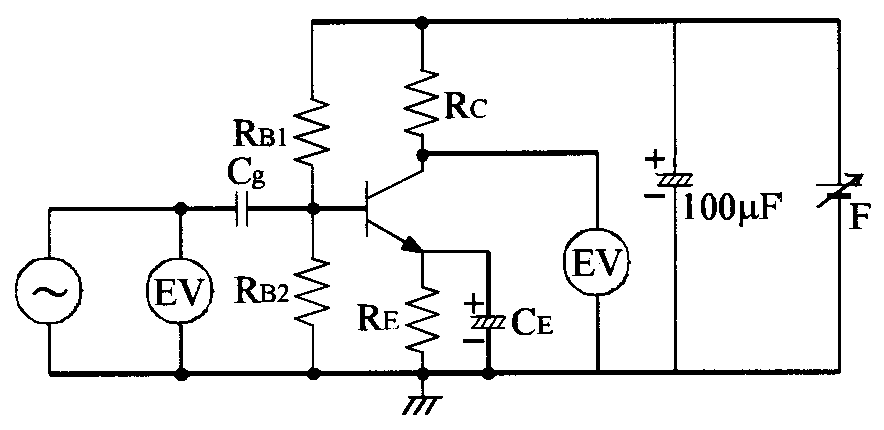
\includegraphics[width=50mm]{fig-13.png}
            \caption{入出力特性測定回路}
            \label{fig:12}
        \end{minipage}
        \begin{minipage}{0.5\hsize}
            \centering
            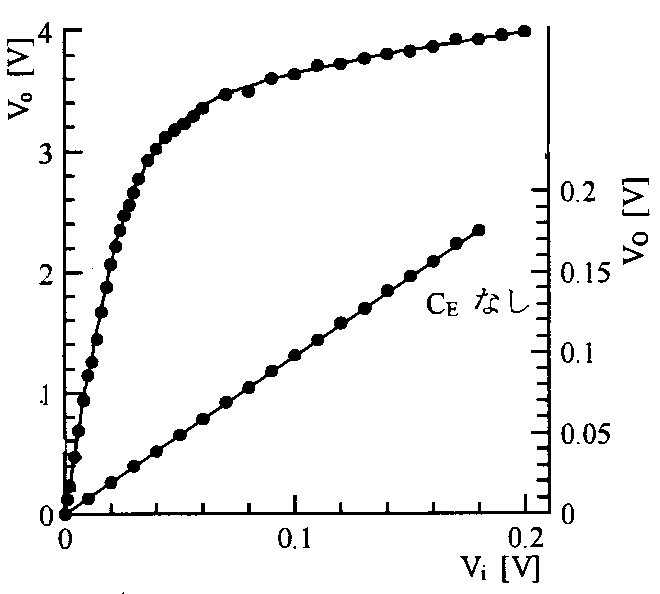
\includegraphics[height=45mm]{fig-14.png}
            \caption{入出力特性}
            \label{fig:13}
        \end{minipage}
    \end{figure}

    \subsubsection{周波数特性の測定}
    設計製作した増幅回路に,低周波発振器より正弦波信号を入力する.
    この入力信号の入力電圧を例えば$e_i = 10[mV]$一定にして,入力信号の周波数を変化させたときの出力電圧の変化を測定する.
    $C_E$の値を変えて同じ測定を行う.
    \begin{figure}[H]
        \begin{minipage}{0.5\hsize}
            \centering
            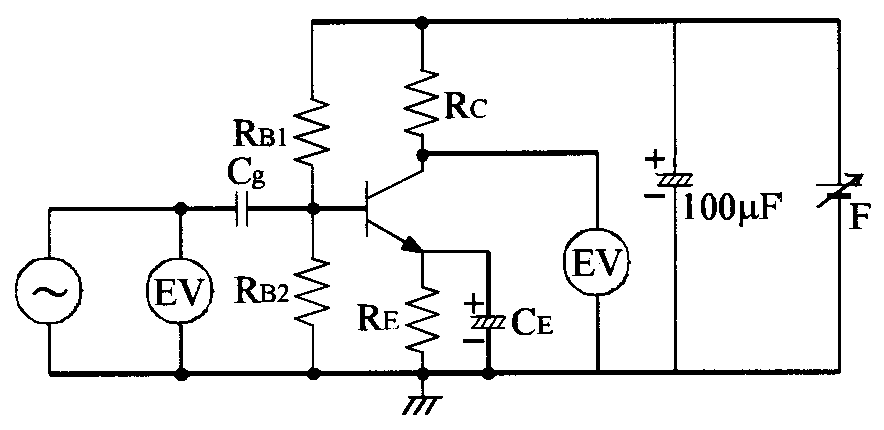
\includegraphics[width=50mm]{fig-15.png}
            \caption{周波数特性測定回路}
            \label{fig:14}
        \end{minipage}
        \begin{minipage}{0.5\hsize}
            \centering
            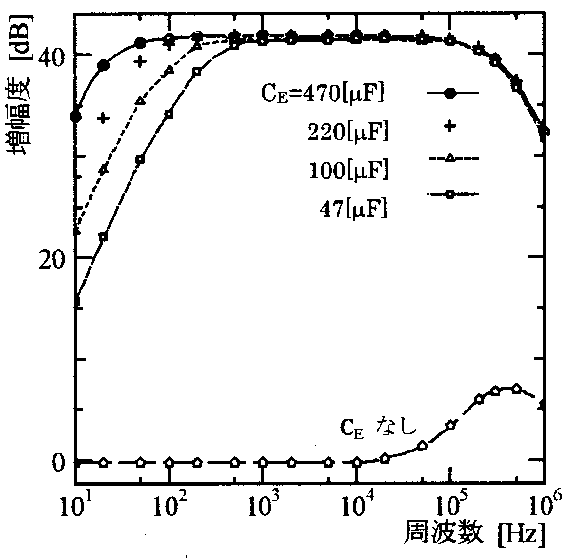
\includegraphics[height=45mm]{fig-16.png}
            \caption{周波数特性}
            \label{fig:15}
        \end{minipage}
    \end{figure}

    \subsubsection{吟味事項}
    \begin{enumerate}
        \item 入出力特性より,制作した増幅回路の増幅度を求める.
        \item バイパスコンデンサ$C_E$のない回路について解析する.測定はしなくていい.
        \item 観測した入力波形および出力波形について,入力特性や増幅特性をもとに考察する.
    \end{enumerate}

    \newpage
    \section{実験結果の処理}
    \subsection{トランジスタの静特性}

    \subsubsection{入力特性の測定結果}
    1.1.1に示した測定を,同一種のトランジスタ3個について,それぞれ行った.
    それぞれを$Tr_1$,$Tr_2$,$Tr_3$と区別することとする.

    以下表\ref{tbl:1}に$Tr_1$の測定結果の表を,図\ref{ex:1}に$Tr_1$の測定結果のグラフを示す.
    \begin{table}[H]
        \centering
        \caption{$Tr_1$の入力特性の測定値}
        \label{tbl:1}
        \small
        \begin{tabular}{|l|l||l|l||l|l|}
        \hline
        \multirow{2}{*}{$V_{BE}[V]$} & $V_{CE}=4[V]$ & \multirow{2}{*}{$V_{BE}[V]$} & $V_{CE}=6[V]$ & \multirow{2}{*}{$V_{BE}[V]$} & $V_{CE}=8[V]$ \\ \cline{2-2} \cline{4-4} \cline{6-6} 
                                & $I_B[\mu A]$   &                         & $I_B[\mu A]$   &                         & $I_B[\mu A]$   \\ \hline
        0                       & 0        & 0                       & 0        & 0                       & 0        \\ \hline
        0.099                   & 0        & 0.562                   & 0.5      & 0.56                    & 0.5      \\ \hline
        0.198                   & 0        & 0.62                    & 2.8      & 0.624                   & 3.8      \\ \hline
        0.297                   & 0        & 0.642                   & 6        & 0.643                   & 7.5      \\ \hline
        0.397                   & 0        & 0.654                   & 10.2     & 0.654                   & 11.4     \\ \hline
        0.493                   & 0.1      & 0.664                   & 15.1     & 0.667                   & 17.4     \\ \hline
        0.555                   & 0.5      & 0.671                   & 20.1     & 0.67                    & 22.2     \\ \hline
        0.589                   & 1.1      & 0.676                   & 25       & 0.672                   & 26.1     \\ \hline
        0.608                   & 1.9      & 0.68                    & 29.9     & 0.675                   & 31.2     \\ \hline
        0.62                    & 2.8      & 0.683                   & 34.8     & 0.656                   & 36       \\ \hline
        0.628                   & 3.8      & 0.686                   & 39.8     &                        &         \\ \hline
        0.634                   & 4.5      & 0.688                   & 44.9     &                        &         \\ \hline
        0.643                   & 6.3      & 0.689                   & 50       &                        &         \\ \hline
        0.646                   & 7.3      &                        &         &                        &         \\ \hline
        0.649                   & 8.2      &                        &         &                        &         \\ \hline
        0.652                   & 9.2      &                        &         &                        &         \\ \hline
        0.66                    & 13       &                        &         &                        &         \\ \hline
        0.665                   & 16.1     &                        &         &                        &         \\ \hline
        0.671                   & 20.1     &                        &         &                        &         \\ \hline
        0.675                   & 24       &                        &         &                        &         \\ \hline
        0.68                    & 28.9     &                        &         &                        &         \\ \hline
        0.685                   & 35.9     &                        &         &                        &         \\ \hline
        0.6866                  & 46.8     &                        &         &                        &         \\ \hline
        0.6887                  & 49.9     &                        &         &                        &         \\ \hline
        \end{tabular}
        \normalsize
    \end{table}
    \begin{figure}[H]
        \centering
        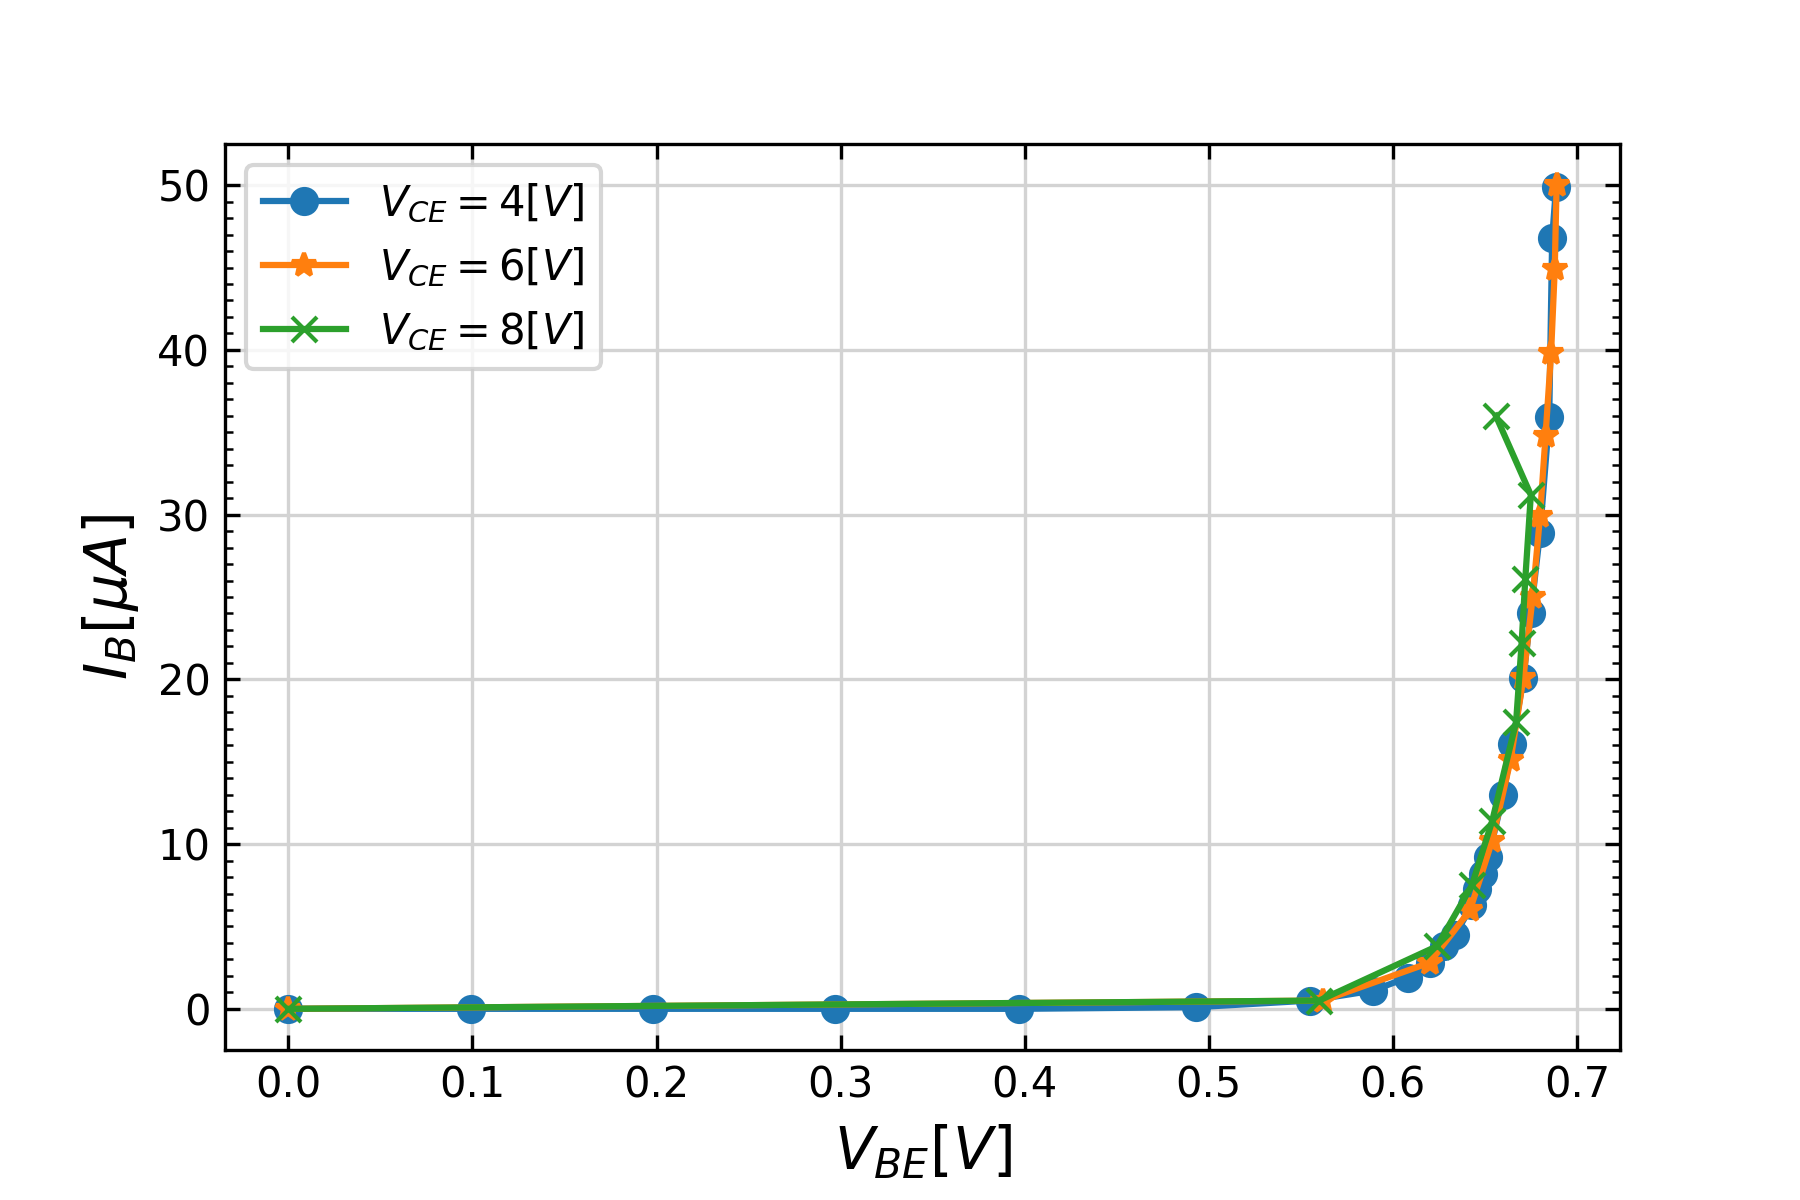
\includegraphics[height=55mm]{ex-1.png}
        \caption{$Tr_1$の入力特性}
        \label{ex:1}    
    \end{figure}
    
    \newpage
    以下表\ref{tbl:2}に$Tr_2$の測定結果の表を,図\ref{ex:2}に$Tr_2$の測定結果のグラフを示す.
    \begin{table}[H]
        \centering
        \caption{$Tr_2$の入力特性の測定値}
        \label{tbl:2}
        \small
        \begin{tabular}{|l|l||l|l||l|l|}
            \hline
            \multirow{2}{*}{$V_{BE}[V]$} & $V_{CE}=4[V]$ & \multirow{2}{*}{$V_{BE}[V]$} & $V_{CE}=6[V]$ & \multirow{2}{*}{$V_{BE}[V]$} & $V_{CE}=8[V]$ \\ \cline{2-2} \cline{4-4} \cline{6-6} 
            & $I_B[\mu A]$   &                         & $I_B[\mu A]$   &                         & $I_B[\mu A]$   \\ \hline
            0     & 0    & 0     & 0    & 0     & 0    \\ \hline
            0.198 & 0    & 0.562 & 0.5  & 0.588 & 1.2  \\ \hline
            0.396 & 0    & 0.618 & 2.7  & 0.633 & 5.5  \\ \hline
            0.559 & 0.5  & 0.643 & 6.5  & 0.652 & 11.2 \\ \hline
            0.609 & 1.9  & 0.657 & 11.2 & 0.661 & 16.2 \\ \hline
            0.639 & 5.5  & 0.667 & 17   & 0.665 & 22.1 \\ \hline
            0.647 & 7.5  & 0.671 & 20.1 & 0.662 & 28   \\ \hline
            0.653 & 9.2  & 0.676 & 24.9 &       &      \\ \hline
            0.66  & 12.1 & 0.68  & 29.9 &       &      \\ \hline
            0.663 & 14.2 & 0.683 & 34.8 &       &      \\ \hline
            0.67  & 21   & 0.686 & 40.6 &       &      \\ \hline
            0.682 & 29.8 & 0.688 & 46.8 &       &      \\ \hline
            0.685 & 34.8 &       &      &       &      \\ \hline
            0.688 & 39.7 &       &      &       &      \\ \hline
            0.69  & 44.8 &       &      &       &      \\ \hline
            0.692 & 49.8 &       &      &       &      \\ \hline
        \end{tabular}
        \normalsize
    \end{table}
    \begin{figure}[H]
        \centering
        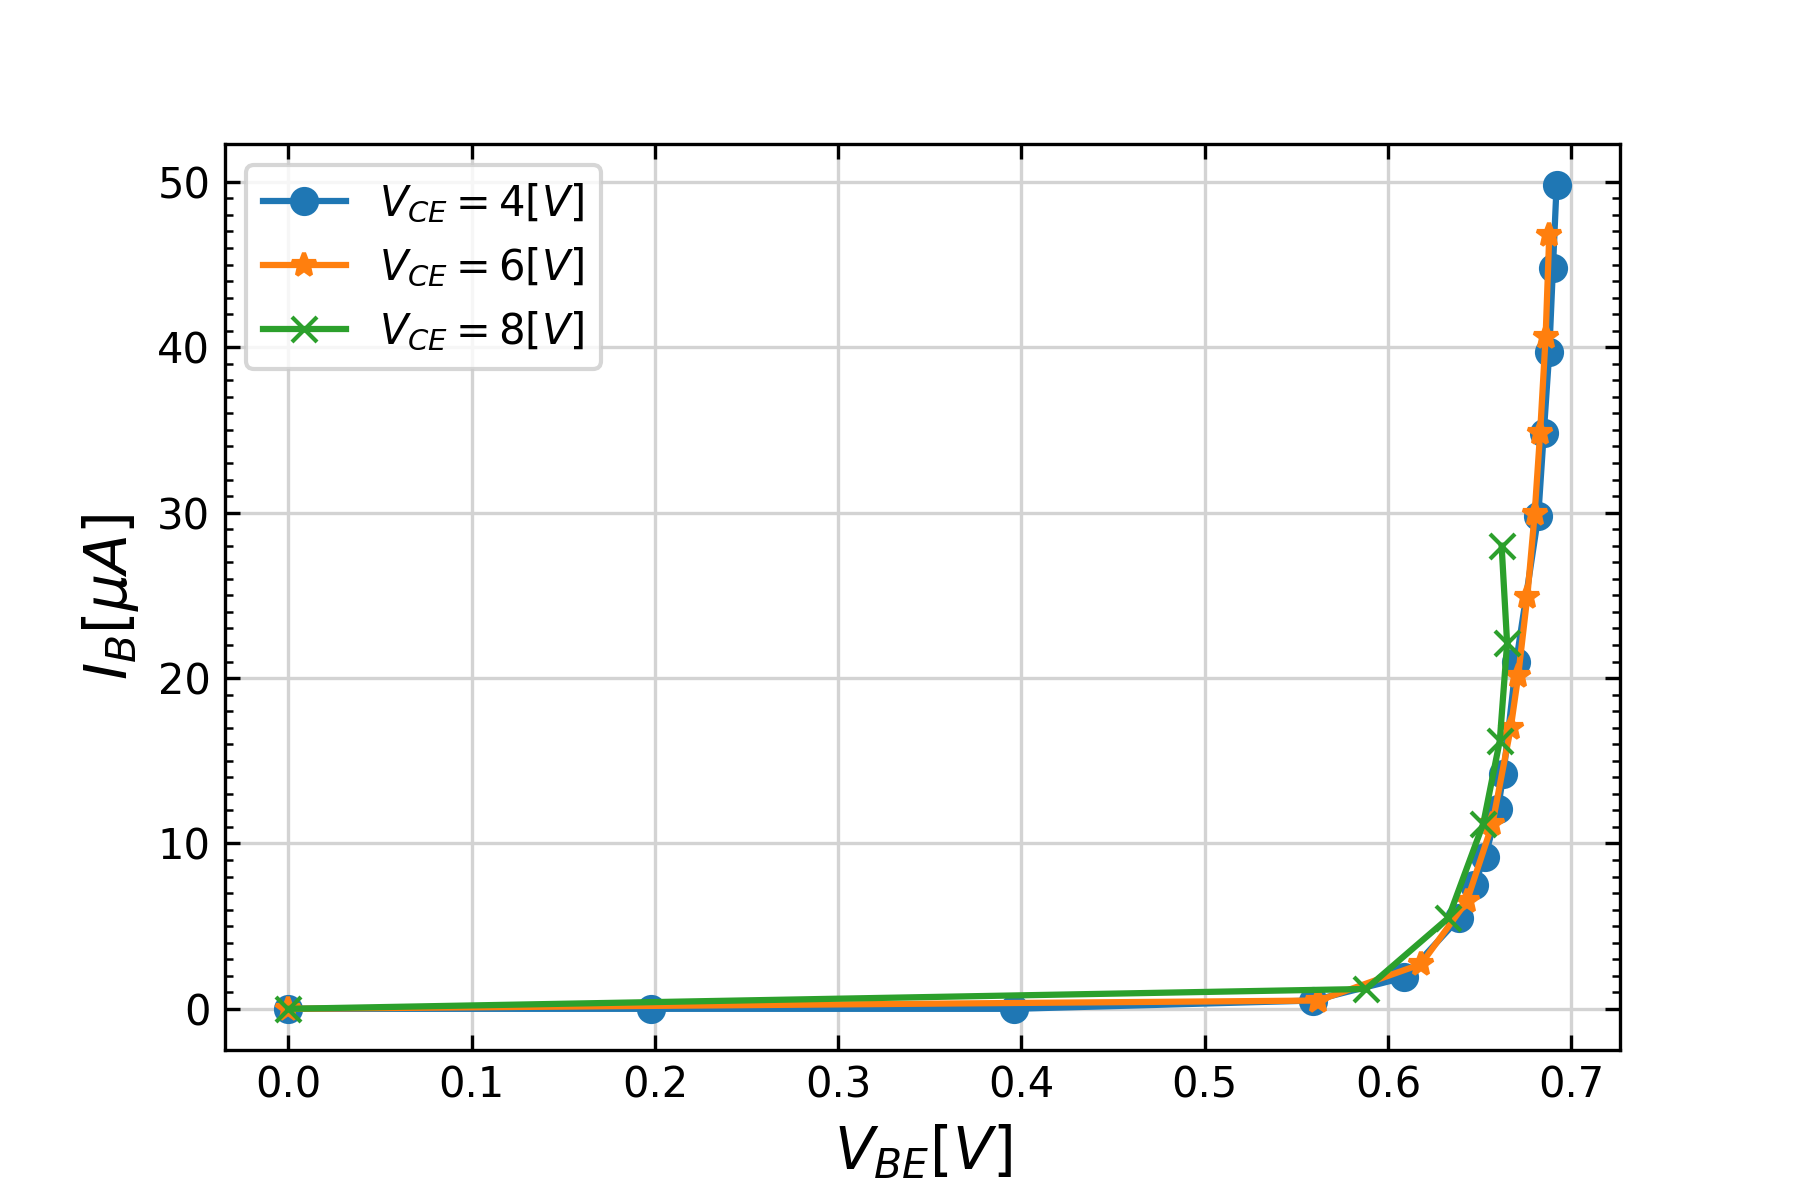
\includegraphics[height=50mm]{ex-2.png}
        \caption{$Tr_2$の入力特性}
        \label{ex:2}    
    \end{figure}

    \newpage
    以下表\ref{tbl:3}に$Tr_3$の測定結果の表を,図\ref{ex:3}に$Tr_3$の測定結果のグラフを示す.
    \begin{table}[H]
        \centering
        \caption{$Tr_3$の入力特性の測定値}
        \label{tbl:3}
        \small
        \begin{tabular}{|l|l||l|l||l|l|}
            \hline
            \multirow{2}{*}{$V_{BE}[V]$} & $V_{CE}=4[V]$ & \multirow{2}{*}{$V_{BE}[V]$} & $V_{CE}=6[V]$ & \multirow{2}{*}{$V_{BE}[V]$} & $V_{CE}=8[V]$ \\ \cline{2-2} \cline{4-4} \cline{6-6} 
            & $I_B[\mu A]$   &                         & $I_B[\mu A]$   &                         & $I_B[\mu A]$   \\ \hline
            0     & 0    & 0     & 0    & 0     & 0    \\ \hline
            0.491 & 0    & 0.562 & 0.5  & 0.561 & 0.5  \\ \hline
            0.59  & 1.1  & 0.619 & 2.8  & 0.64  & 6.5  \\ \hline
            0.63  & 5.5  & 0.632 & 4.5  & 0.655 & 12.2 \\ \hline
            0.653 & 10.3 & 0.653 & 10.2 & 0.656 & 17.1 \\ \hline
            0.663 & 15.1 & 0.662 & 15.1 & 0.671 & 24.1 \\ \hline
            0.671 & 20.5 & 0.669 & 20.1 & 0.675 & 29.1 \\ \hline
            0.676 & 25   & 0.673 & 25   & 0.672 & 35   \\ \hline
            0.68  & 29.9 & 0.676 & 30   &       &      \\ \hline
            0.684 & 34.8 & 0.678 & 34.9 &       &      \\ \hline
            0.687 & 39.8 & 0.679 & 39.8 &       &      \\ \hline
            0.689 & 44.8 & 0.68  & 50   &       &      \\ \hline
            0.691 & 49.9 &       &      &       &      \\ \hline
        \end{tabular}
        \normalsize
    \end{table}
    \begin{figure}[H]
        \centering
        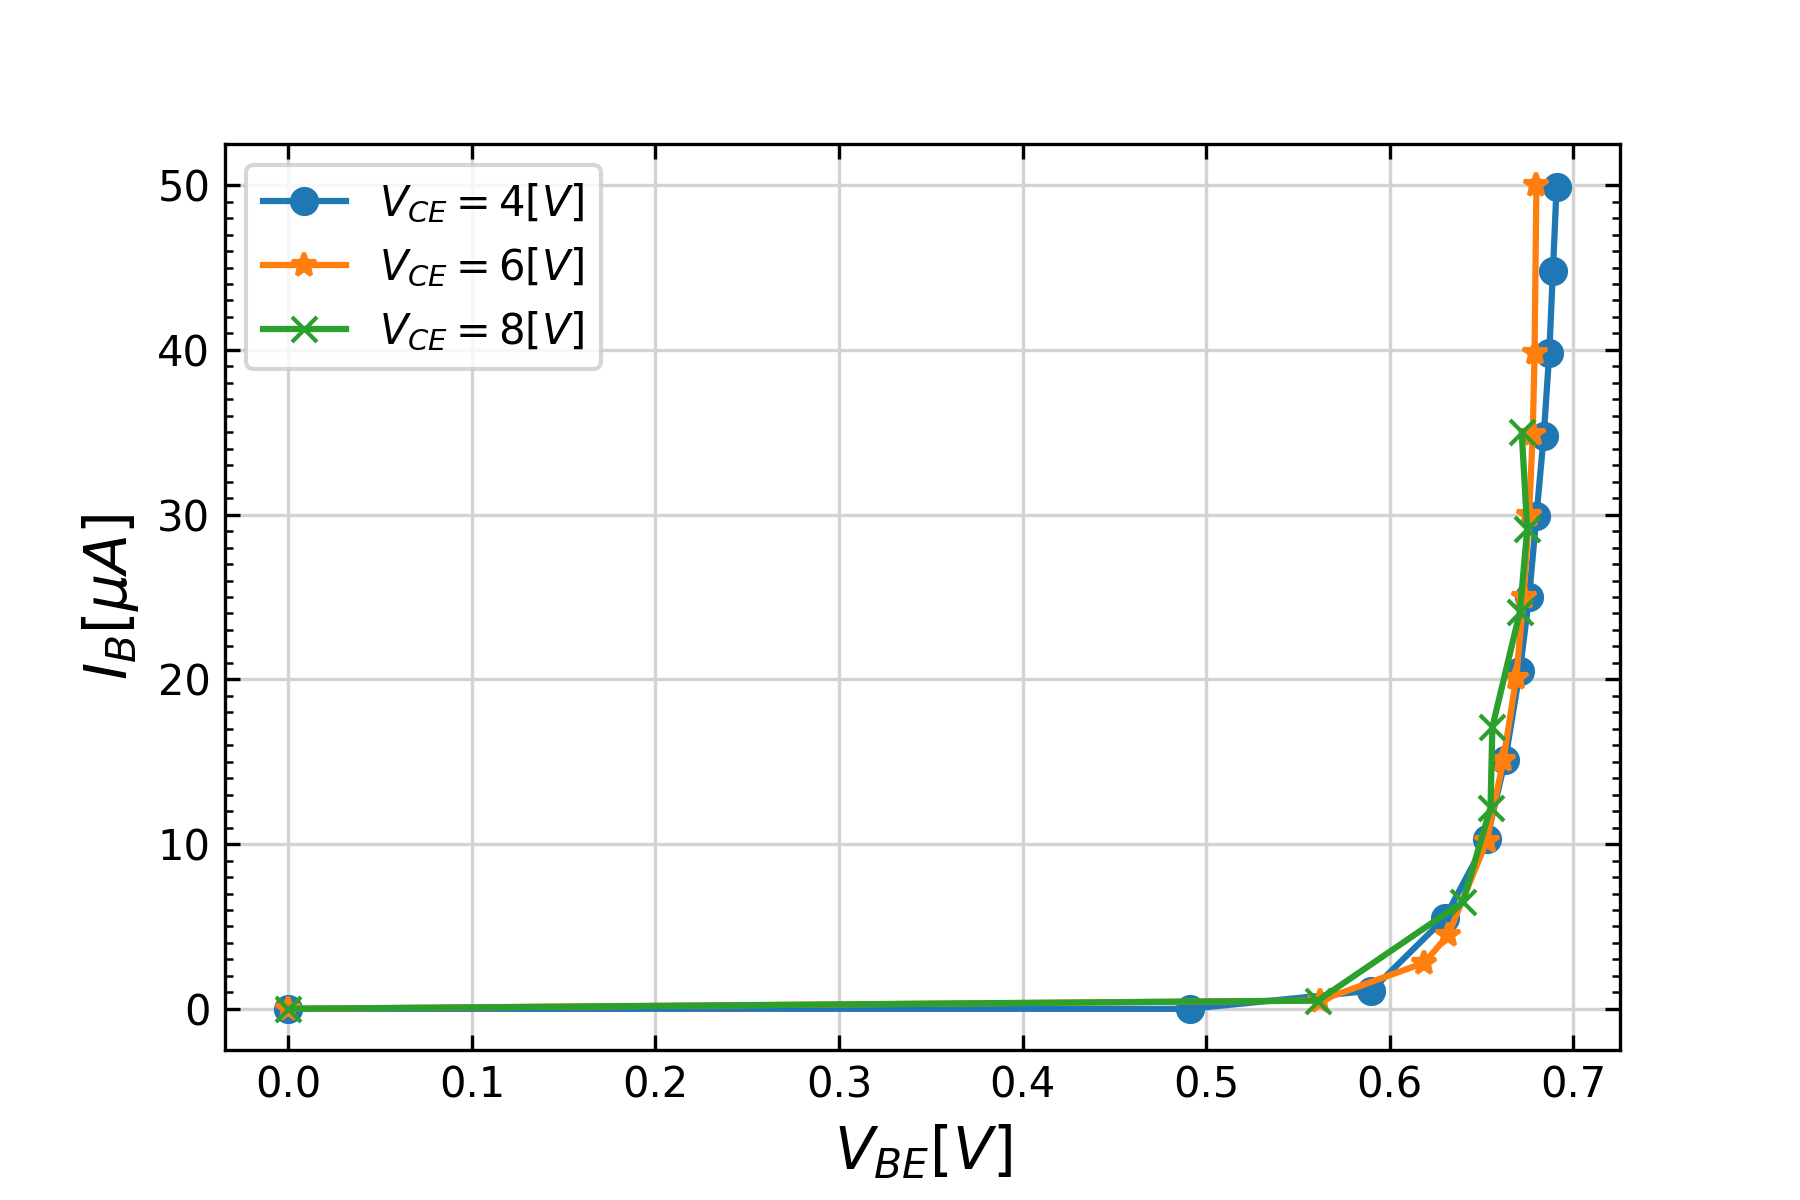
\includegraphics[height=50mm]{ex-3.png}
        \caption{$Tr_3$の入力特性}
        \label{ex:3}
    \end{figure}

    \newpage
    \subsubsection{出力特性の測定結果}
    1.1.2に示した測定を,2.1.1に示した測定と同様に同一種のトランジスタ3個について,それぞれ行った.
    以下,表\ref{tbl:4}に$Tr_1$の測定結果の表を,図\ref{ex:4}の測定結果のグラフを示す.
    \begin{table}[H]
        \centering
        \caption{$Tr_1$の出力特性の測定値}
        \label{tbl:4}
        \small
        \begin{tabular}{|l|l|l|l|l|l|l|l|}
            \hline
            \multirow{2}{*}{$V_{CE}$} & $I_B=0[\mu A]$ & \multirow{2}{*}{$V_{CE}$} & $I_B=5[\mu A]$ & \multirow{2}{*}{$V_{CE}$} & $I_B=10[\mu A]$ & \multirow{2}{*}{$V_{CE}$} & $I_B=20[\mu A]$ \\ \cline{2-2} \cline{4-4} \cline{6-6} \cline{8-8} 
            & $I_C[mA]$      &                           & $I_C[mA]$      &                           & $I_C[mA]$       &                           & $I_C[mA]$       \\ \hline
            0                         & 0              & 0                         & 0              & 0                         & 0               & 0                         & 0               \\ \hline
            1.001                     & 0              & 0.005                     & 0              & 0.006                     & 0               & 0.006                     & 0               \\ \hline
            2.001                     & 0              & 0.099                     & 0.238          & 0.068                     & 0.26            & 0.074                     & 0.68            \\ \hline
            3                         & 0              & 0.17                      & 0.618          & 0.107                     & 0.71            & 0.124                     & 1.88            \\ \hline
            4                         & 0              & 0.21                      & 0.68           & 0.145                     & 1.17            & 0.183                     & 2.9             \\ \hline
            5                         & 0              & 0.308                     & 0.7            & 0.205                     & 1.47            & 0.272                     & 3.18            \\ \hline
            6                         & 0              & 0.408                     & 0.7            & 0.298                     & 1.52            & 0.371                     & 3.2             \\ \hline
            7                         & 0              & 0.508                     & 0.7            & 0.398                     & 1.52            & 0.471                     & 3.2             \\ \hline
            8                         & 0              & 1.508                     & 0.71           & 0.497                     & 1.53            & 0.571                     & 3.2             \\ \hline
            9                         & 0              & 2.506                     & 0.71           & 0.597                     & 1.53            & 1.57                      & 3.2             \\ \hline
            10                        & 0              & 3.506                     & 0.72           & 1.596                     & 1.54            & 2.568                     & 3.22            \\ \hline
            11                        & 0              & 4.51                      & 0.72           & 2.595                     & 1.55            & 3.567                     & 3.23            \\ \hline
            12                        & 0              & 6.5                       & 0.72           & 3.593                     & 1.55            & 4.57                      & 3.24            \\ \hline
            13                        & 0              & 8.5                       & 0.73           & 4.59                      & 1.56            & 6.56                      & 3.26            \\ \hline
            14                        & 0              & 10.5                      & 0.74           & 6.59                      & 1.58            & 8.56                      & 3.39            \\ \hline
            15                        & 0              & 12.5                      & 0.74           & 8.59                      & 1.59            & 10.56                     & 3.4             \\ \hline
            16                        & 0              & 14.5                      & 0.75           & 10.59                     & 1.6             & 12.56                     & 3.46            \\ \hline
                                      & 0              & 16.5                      & 0.75           & 12.58                     & 1.61            & 14.56                     & 3.5             \\ \hline
                                      &                &                           &                & 14.58                     & 1.63            & 16.55                     & 3.58            \\ \hline
                                      &                &                           &                & 16.58                     & 1.66            &                           &                 \\ \hline
                                      &                &                           &                &                           &                 &                           &                 \\ \hline
            \end{tabular}
        \normalsize
    \end{table}
    \begin{table}[H]
        \centering
        \begin{tabular}{|l|l||l|l||l|l|}
        \hline
        \multirow{2}{*}{$V_{CE}$} & $I_B=30[\mu A]$ & \multirow{2}{*}{$V_{CE}$} & $I_B=40[\mu A]$ & \multirow{2}{*}{$V_{CE}$} & $I_B=50[\mu A]$ \\ \cline{2-2} \cline{4-4} \cline{6-6} 
        & $I_C[mA]$       &                           & $I_C[mA]$       &                           & $I_C[mA]$       \\ \hline
        0                         & 0               & 0                         & 0               & 0                         & 0               \\ \hline
        0.006                     & 0               & 0.006                     & 0               & 0.005                     & 0               \\ \hline
        0.788                     & 5.12            & 0.715                     & 6.88            & 0.643                     & 8.6             \\ \hline
        1.788                     & 5.16            & 1.715                     & 6.88            & 1.643                     & 8.62            \\ \hline
        2.787                     & 5.18            & 2.713                     & 6.92            & 2.641                     & 8.68            \\ \hline
        3.785                     & 5.2             & 3.712                     & 6.96            & 3.639                     & 8.72            \\ \hline
        4.79                      & 5.22            & 4.71                      & 7.02            & 4.64                      & 8.8             \\ \hline
        6.78                      & 5.3             & 6.7                       & 7.12            & 6.63                      & 8.98            \\ \hline
        8.78                      & 5.4             & 8.7                       & 7.28            & 8.62                      & 9.2             \\ \hline
        10.77                     & 5.48            & 10.69                     & 7.4             & 10.61                     & 9.4             \\ \hline
        12.77                     & 5.6             & 12.69                     & 7.58            & 12.6                      & 9.56            \\ \hline
        14.76                     & 5.72            & 14.68                     & 7.78            & 14.58                     & 10              \\ \hline
        16.76                     & 5.82            & 16.67                     & 7.96            & 16.57                     & 10.35           \\ \hline
        \end{tabular}
    \end{table}
    \begin{figure}[H]
        \centering
        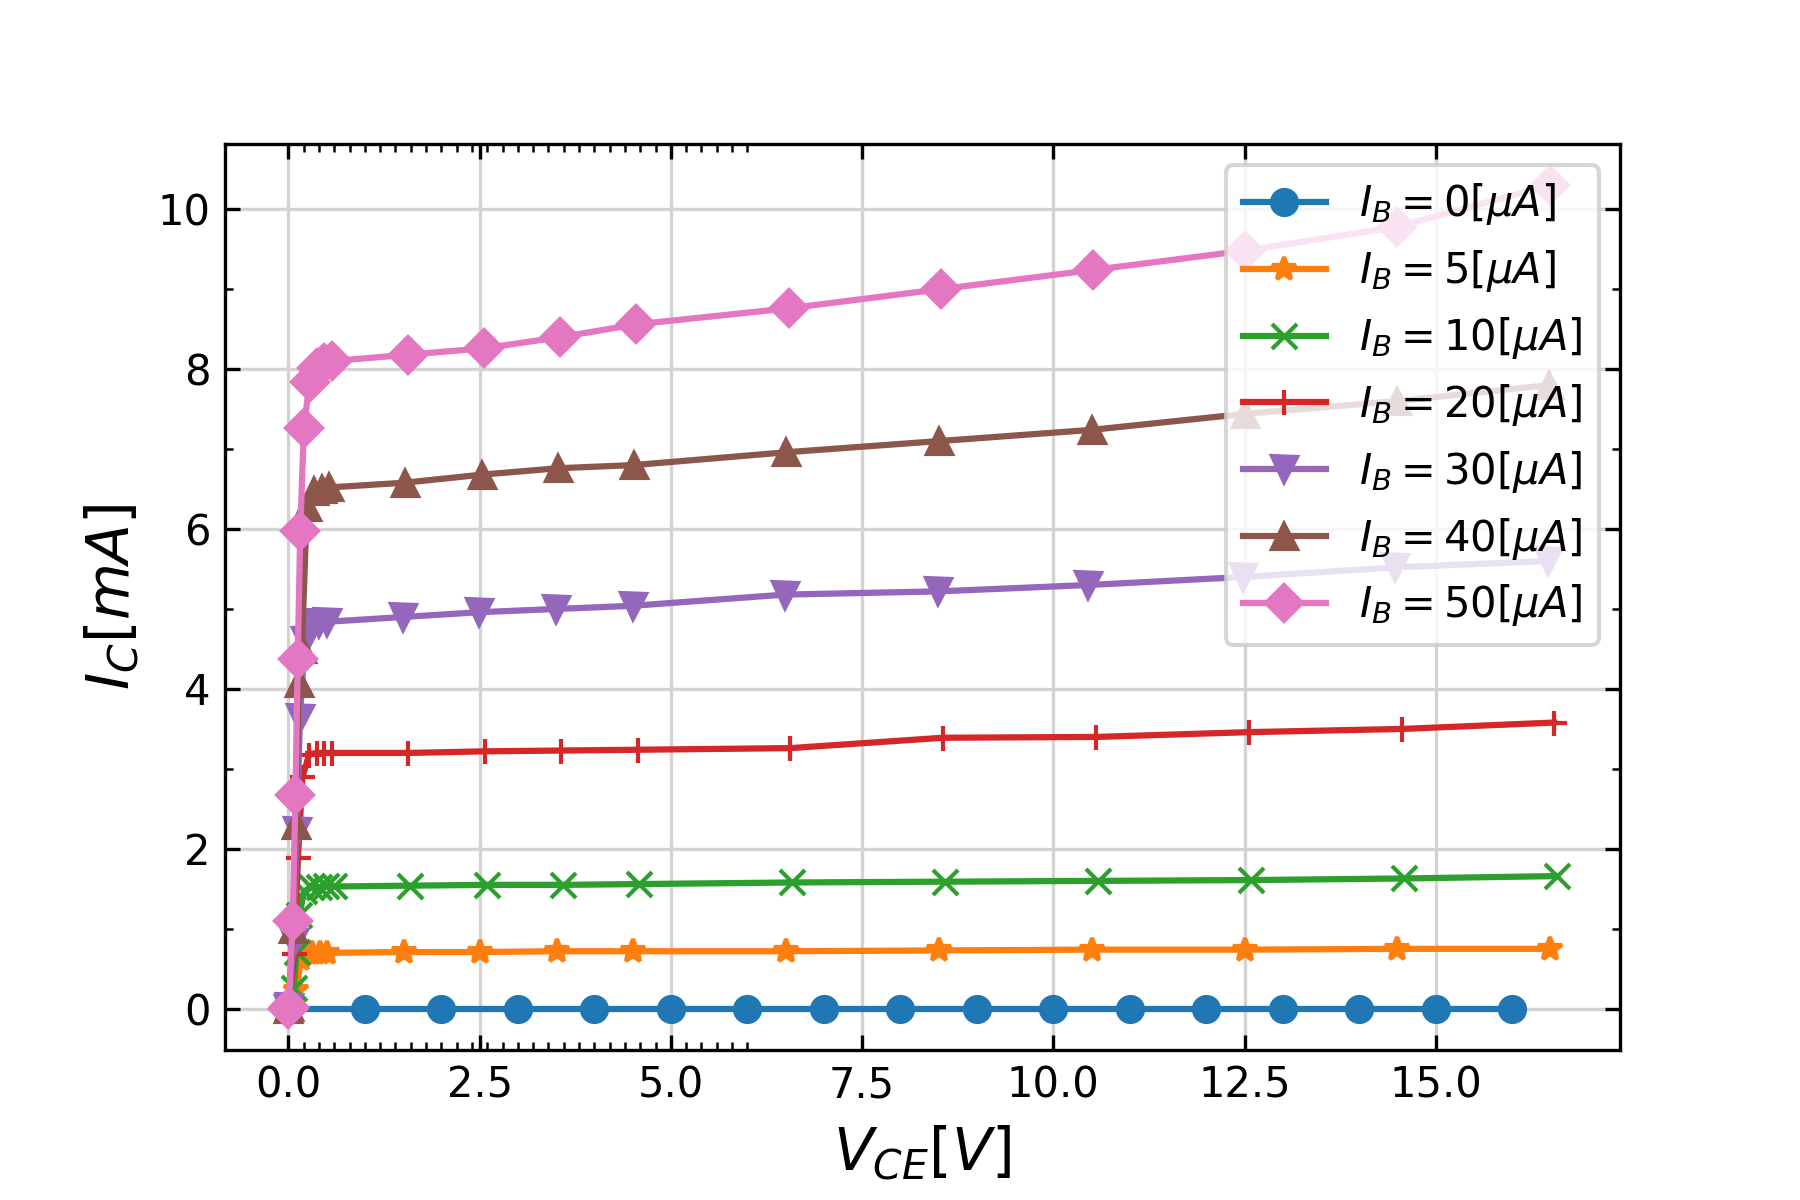
\includegraphics[height=50mm]{ex-4.png}
        \caption{$Tr_1$の出力特性}
        \label{ex:4}
    \end{figure}

    \newpage
    以下,表\ref{tbl:5}に$Tr_2$の測定結果の表を,図\ref{ex:5}の測定結果のグラフを示す.
    \begin{table}[H]
        \centering
        \caption{$Tr_2$の出力特性の測定値}
        \label{tbl:5}
        \small
        \begin{tabular}{|l|l|l|l|l|l|l|l|}
        \hline
        \multirow{2}{*}{$V_{CE}$} & $I_B=0[\mu A]$ & \multirow{2}{*}{$V_{CE}$} & $I_B=5[\mu A]$ & \multirow{2}{*}{$V_{CE}$} & $I_B=10[\mu A]$ & \multirow{2}{*}{$V_{CE}$} & $I_B=20[\mu A]$ \\ \cline{2-2} \cline{4-4} \cline{6-6} \cline{8-8} 
        & $I_C[mA]$      &                           & $I_C[mA]$      &                           & $I_C[mA]$       &                           & $I_C[mA]$       \\ \hline            
        0                         & 0              & 0                         & 0              & 0                         & 0               & 0                         & 0               \\ \hline
        1.001                     & 0              & 0.004                     & 0              & 0.006                     & 0               & 0.006                     & 0               \\ \hline
        2.001                     & 0              & 0.737                     & 0.7            & 0.79                      & 1.56            & 0.855                     & 3.52            \\ \hline
        3                         & 0              & 1.735                     & 0.704          & 1.789                     & 1.57            & 1.853                     & 3.56            \\ \hline
        4                         & 0              & 2.733                     & 0.708          & 2.789                     & 1.58            & 2.53                      & 3.58            \\ \hline
        5                         & 0              & 3.732                     & 0.712          & 3.787                     & 1.59            & 3.852                     & 3.6             \\ \hline
        6                         & 0              & 4.73                      & 0.716          & 4.79                      & 1.6             & 4.85                      & 3.62            \\ \hline
        7                         & 0              & 6.73                      & 0.72           & 6.78                      & 1.62            & 6.85                      & 3.68            \\ \hline
        8                         & 0              & 8.73                      & 0.728          & 8.78                      & 1.63            & 8.85                      & 3.7             \\ \hline
        9                         & 0              & 10.72                     & 0.732          & 10.8                      & 1.64            & 10.84                     & 3.8             \\ \hline
        10                        & 0              & 12.72                     & 0.738          & 12.78                     & 1.65            & 12.84                     & 3.88            \\ \hline
        11                        & 0              & 14.72                     & 0.74           & 14.78                     & 1.66            & 14.84                     & 3.92            \\ \hline
        12                        & 0              & 16.72                     & 0.744          & 16.77                     & 1.68            & 16.83                     & 3.96            \\ \hline
        13                        & 0              &                           &                &                           &                 &                           &                 \\ \hline
        14                        & 0              &                           &                &                           &                 &                           &                 \\ \hline
        15                        & 0              &                           &                &                           &                 &                           &                 \\ \hline
        16                        & 0              &                           &                &                           &                 &                           &                 \\ \hline
        \end{tabular}
        \normalsize
    \end{table}
    \begin{table}[H]
        \centering
        \begin{tabular}{|l|l||l|l||l|l|}
        \hline
        \multirow{2}{*}{$V_{CE}$} & $I_B=30[\mu A]$ & \multirow{2}{*}{$V_{CE}$} & $I_B=40[\mu A]$ & \multirow{2}{*}{$V_{CE}$} & $I_B=50[\mu A]$ \\ \cline{2-2} \cline{4-4} \cline{6-6} 
        & $I_C[mA]$       &                           & $I_C[mA]$       &                           & $I_C[mA]$       \\ \hline
        0                         & 0               & 0                         & 0               & 0                         & 0               \\ \hline
        0.006                     & 0               & 0.006                     & 0               & 0.005                     & 0               \\ \hline
        0.788                     & 5.12            & 0.715                     & 6.88            & 0.643                     & 8.6             \\ \hline
        1.788                     & 5.16            & 1.715                     & 6.88            & 1.643                     & 8.62            \\ \hline
        2.787                     & 5.18            & 2.713                     & 6.92            & 2.641                     & 8.68            \\ \hline
        3.785                     & 5.2             & 3.712                     & 6.96            & 3.639                     & 8.72            \\ \hline
        4.79                      & 5.22            & 4.71                      & 7.02            & 4.64                      & 8.8             \\ \hline
        6.78                      & 5.3             & 6.7                       & 7.12            & 6.63                      & 8.98            \\ \hline
        8.78                      & 5.4             & 8.7                       & 7.28            & 8.62                      & 9.2             \\ \hline
        10.77                     & 5.48            & 10.69                     & 7.4             & 10.61                     & 9.4             \\ \hline
        12.77                     & 5.6             & 12.69                     & 7.58            & 12.6                      & 9.56            \\ \hline
        14.76                     & 5.72            & 14.68                     & 7.78            & 14.58                     & 10              \\ \hline
        16.76                     & 5.82            & 16.67                     & 7.96            & 16.57                     & 10.35           \\ \hline
        \end{tabular}
    \end{table}
    \begin{figure}[H]
        \centering
        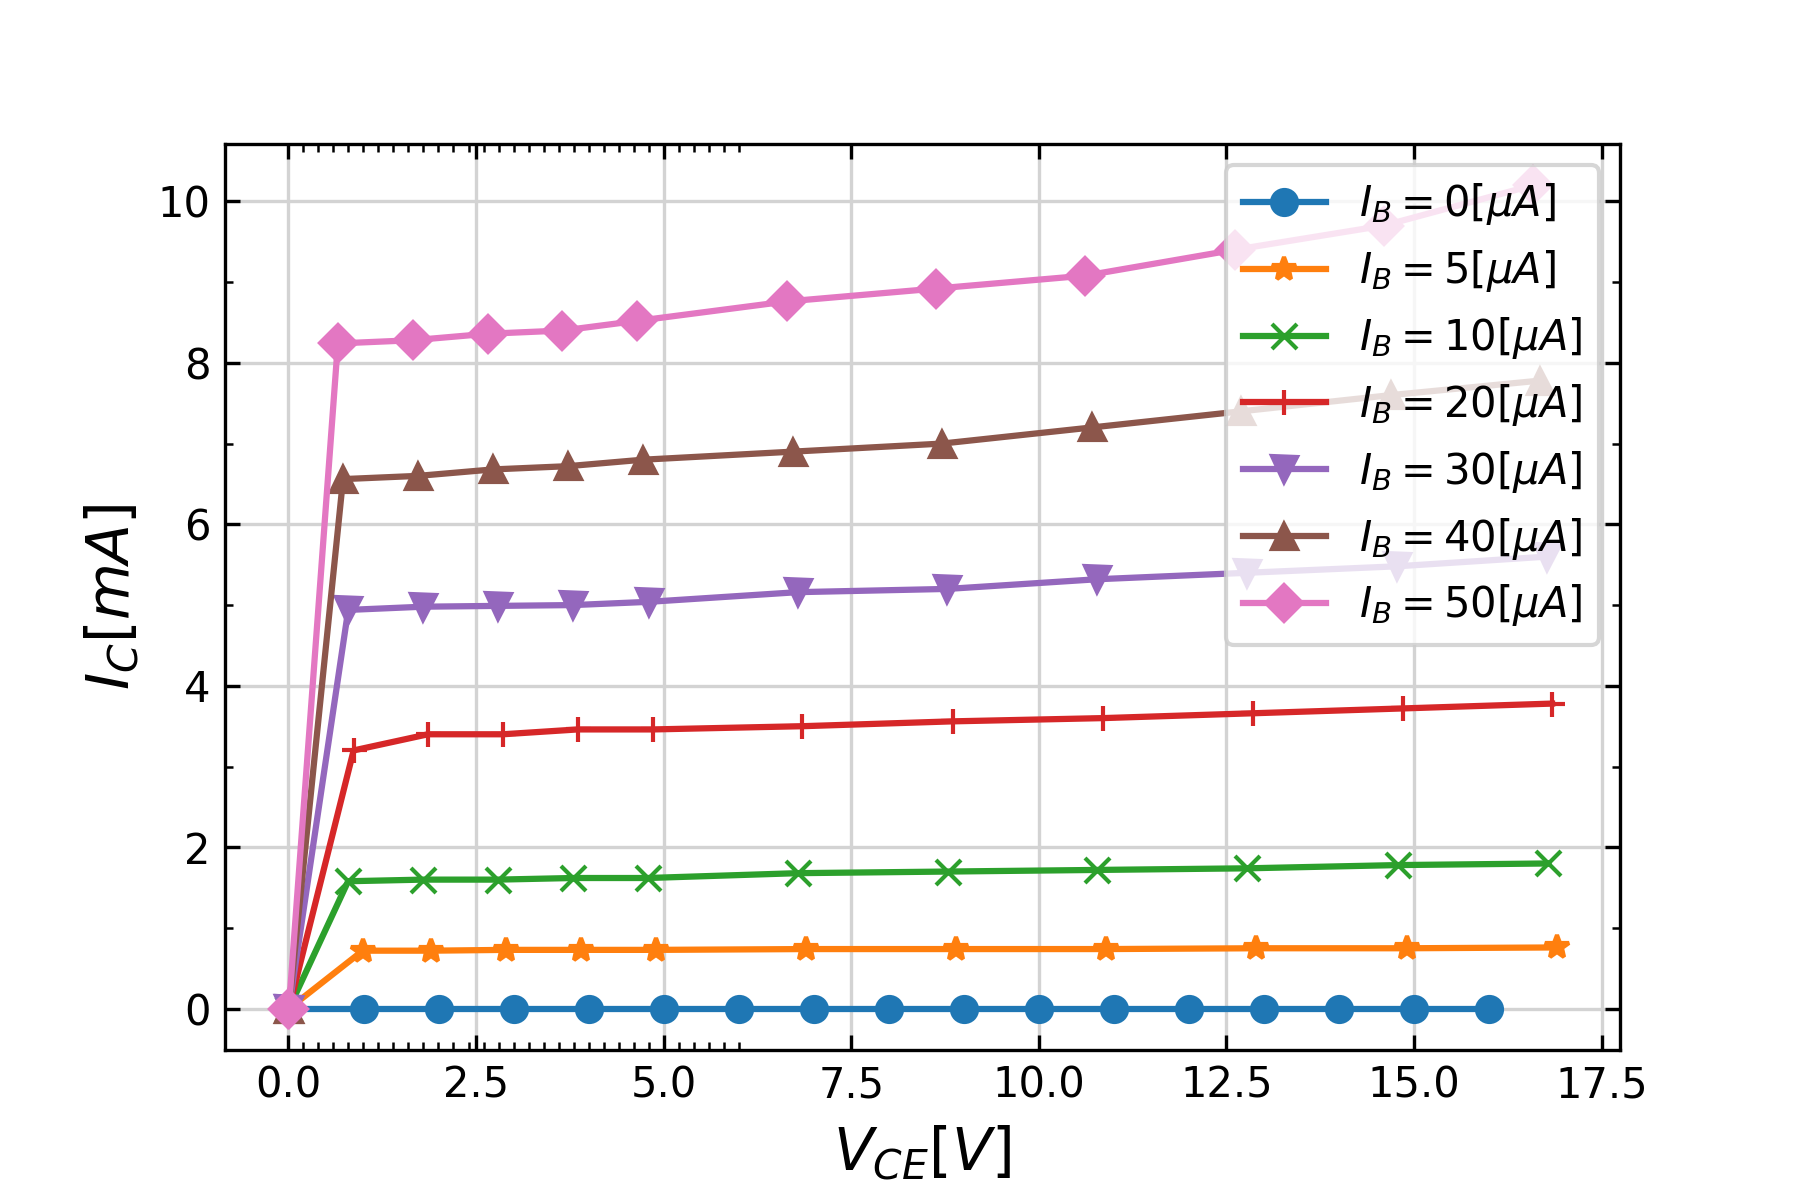
\includegraphics[height=50mm]{ex-5.png}
        \caption{$Tr_2$の出力特性}
        \label{ex:5}
    \end{figure}

    \newpage
    以下,表\ref{tbl:6}に$Tr_3$の測定結果の表を,図\ref{ex:6}の測定結果のグラフを示す.
    \begin{table}[H]
        \centering
        \caption{$Tr_3$の出力特性の測定値}
        \label{tbl:6}
        \small
        \begin{tabular}{|l|l||l|l||l|l||l|l|}
        \hline
        \multirow{2}{*}{$V_{CE}$} & $I_B=0[\mu A]$ & \multirow{2}{*}{$V_{CE}$} & $I_B=5[\mu A]$ & \multirow{2}{*}{$V_{CE}$} & $I_B=10[\mu A]$ & \multirow{2}{*}{$V_{CE}$} & $I_B=20[\mu A]$ \\ \cline{2-2} \cline{4-4} \cline{6-6} \cline{8-8} 
                                    & $I_C[mA]$      &                           & $I_C[mA]$      &                           & $I_C[mA]$       &                           & $I_C[mA]$       \\ \hline
        0                         & 0              & 0                         & 0              & 0                         & 0               & 0                         & 0               \\ \hline
        1.001                     & 0              & 0.004                     & 0              & 0.006                     & 0               & 0.006                     & 0               \\ \hline
        2.001                     & 0              & 0.737                     & 0.7            & 0.79                      & 1.56            & 0.855                     & 3.52            \\ \hline
        3                         & 0              & 1.735                     & 0.704          & 1.789                     & 1.57            & 1.853                     & 3.56            \\ \hline
        4                         & 0              & 2.733                     & 0.708          & 2.789                     & 1.58            & 2.53                      & 3.58            \\ \hline
        5                         & 0              & 3.732                     & 0.712          & 3.787                     & 1.59            & 3.852                     & 3.6             \\ \hline
        6                         & 0              & 4.73                      & 0.716          & 4.79                      & 1.6             & 4.85                      & 3.62            \\ \hline
        7                         & 0              & 6.73                      & 0.72           & 6.78                      & 1.62            & 6.85                      & 3.68            \\ \hline
        8                         & 0              & 8.73                      & 0.728          & 8.78                      & 1.63            & 8.85                      & 3.7             \\ \hline
        9                         & 0              & 10.72                     & 0.732          & 10.8                      & 1.64            & 10.84                     & 3.8             \\ \hline
        10                        & 0              & 12.72                     & 0.738          & 12.78                     & 1.65            & 12.84                     & 3.88            \\ \hline
        11                        & 0              & 14.72                     & 0.74           & 14.78                     & 1.66            & 14.84                     & 3.92            \\ \hline
        12                        & 0              & 16.72                     & 0.744          & 16.77                     & 1.68            & 16.83                     & 3.96            \\ \hline
        13                        & 0              &                           &                &                           &                 &                           &                 \\ \hline
        14                        & 0              &                           &                &                           &                 &                           &                 \\ \hline
        15                        & 0              &                           &                &                           &                 &                           &                 \\ \hline
        16                        & 0              &                           &                &                           &                 &                           &                 \\ \hline
        \end{tabular}
    \end{table}
    \begin{table}[H]
        \centering
        \begin{tabular}{|l|l||l|l||l|l|}
        \hline
        \multirow{2}{*}{$V_{CE}$} & $I_B=30[\mu A]$ & \multirow{2}{*}{$V_{CE}$} & $I_B=40[\mu A]$ & \multirow{2}{*}{$V_{CE}$} & $I_B=50[\mu A]$ \\ \cline{2-2} \cline{4-4} \cline{6-6} 
                                  & $I_C[mA]$       &                           & $I_C[mA]$       &                           & $I_C[mA]$       \\ \hline
        0                         & 0               & 0                         & 0               & 0                         & 0               \\ \hline
        0.006                     & 0               & 0.006                     & 0               & 0.005                     & 0               \\ \hline
        0.788                     & 5.12            & 0.715                     & 6.88            & 0.643                     & 8.6             \\ \hline
        1.788                     & 5.16            & 1.715                     & 6.88            & 1.643                     & 8.62            \\ \hline
        2.787                     & 5.18            & 2.713                     & 6.92            & 2.641                     & 8.68            \\ \hline
        3.785                     & 5.2             & 3.712                     & 6.96            & 3.639                     & 8.72            \\ \hline
        4.79                      & 5.22            & 4.71                      & 7.02            & 4.64                      & 8.8             \\ \hline
        6.78                      & 5.3             & 6.7                       & 7.12            & 6.63                      & 8.98            \\ \hline
        8.78                      & 5.4             & 8.7                       & 7.28            & 8.62                      & 9.2             \\ \hline
        10.77                     & 5.48            & 10.69                     & 7.4             & 10.61                     & 9.4             \\ \hline
        12.77                     & 5.6             & 12.69                     & 7.58            & 12.6                      & 9.56            \\ \hline
        14.76                     & 5.72            & 14.68                     & 7.78            & 14.58                     & 10              \\ \hline
        16.76                     & 5.82            & 16.67                     & 7.96            & 16.57                     & 10.35           \\ \hline
        \end{tabular}
    \end{table}
    \begin{figure}[H]
        \centering
        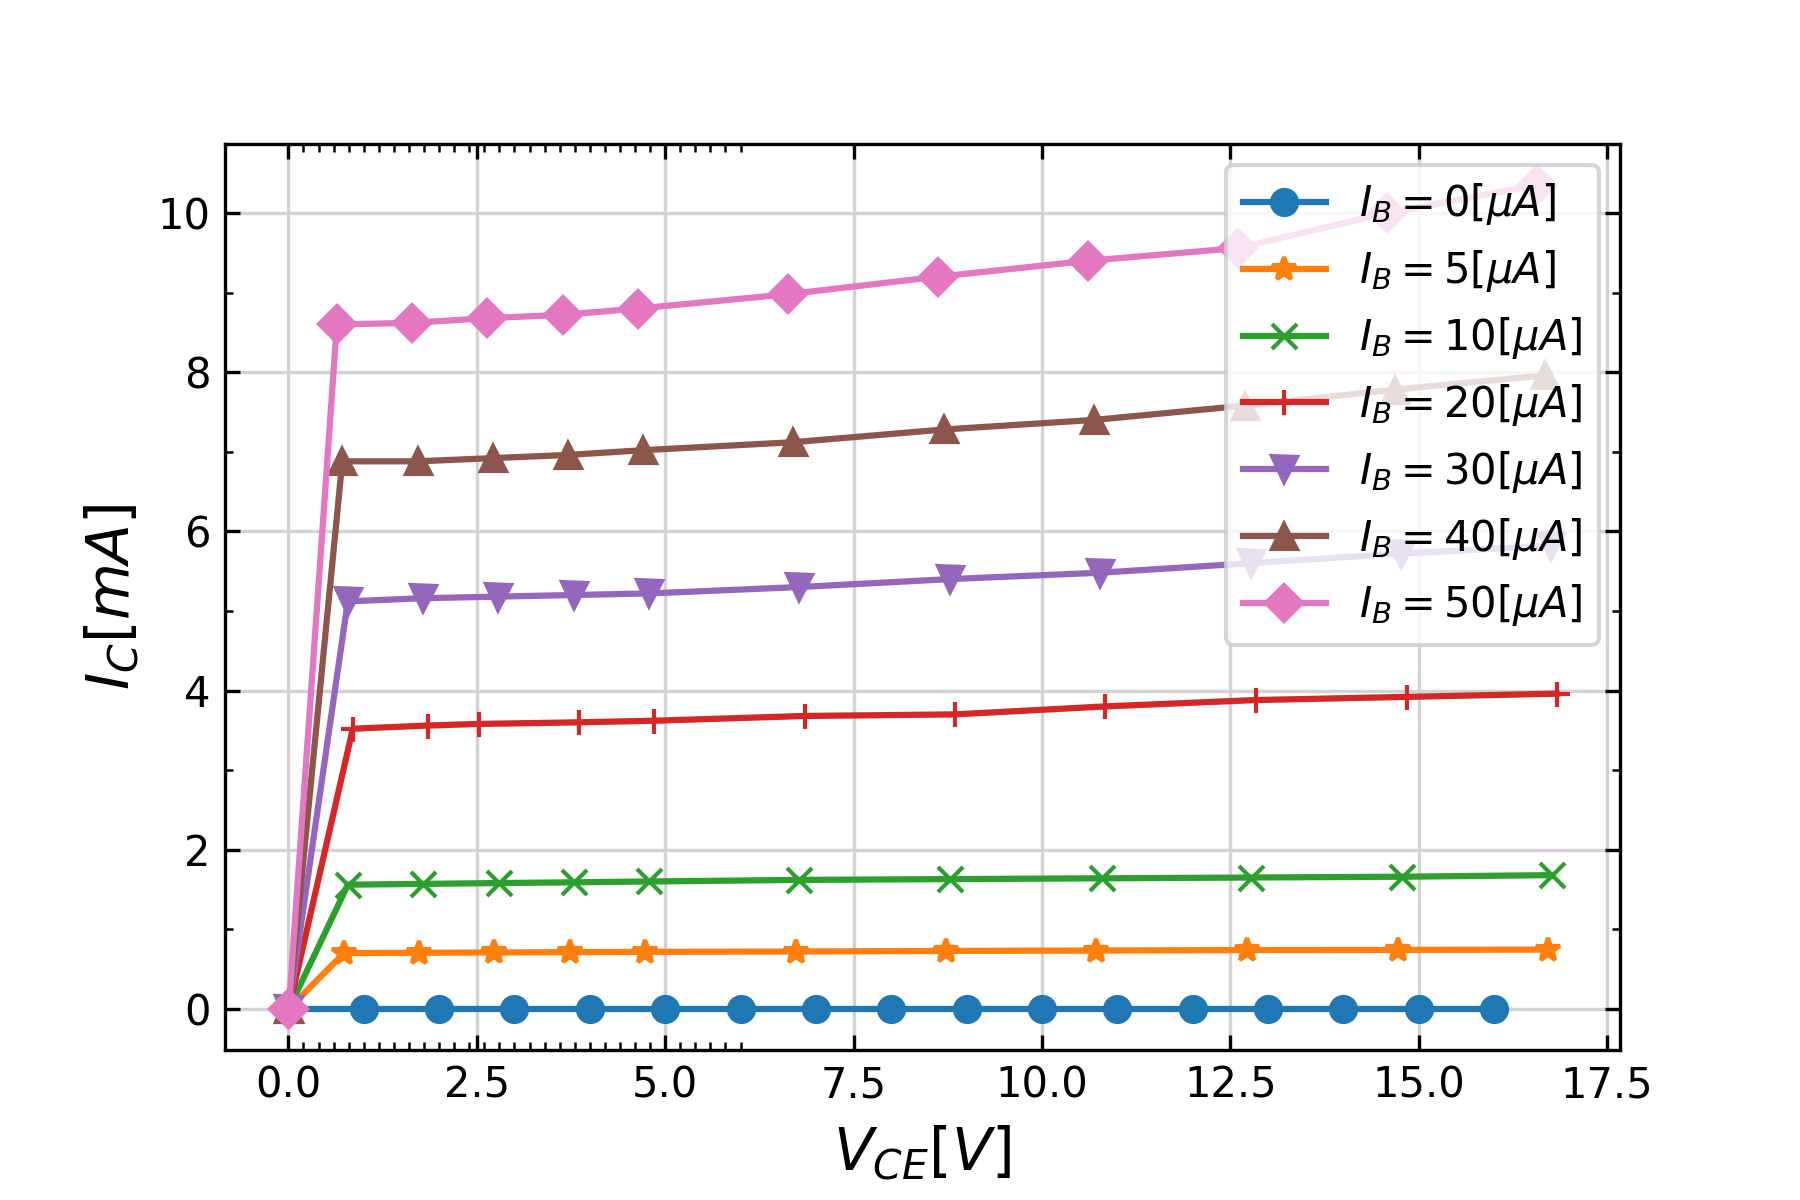
\includegraphics[height=50mm]{ex-6.png}
        \caption{$Tr_3$の出力特性}
        \label{ex:6}
    \end{figure}

    \newpage
    \subsection{トランジスタ増幅}
    \subsubsection{電流増幅特性の測定方法}
    1.2.1に示した測定を,2.1.1に示した測定と同様に同一種のトランジスタ3個について,それぞれ行った.
    以下,表\ref{tbl:7}に$Tr_1$の測定結果の表を,図\ref{ex:7}の測定結果のグラフを示す.
    \begin{table}[H]
        \centering
        \caption{$Tr_1$の電流増幅特性の測定値}
        \label{tbl:7}
        \small
        \begin{tabular}{|l|l|}
        \hline
        $I_B[\mu A]$ & $I_C[mA]$ \\ \hline
        0            & 0         \\ \hline
        10           & 1.78      \\ \hline
        20           & 3.48      \\ \hline
        30           & 5.19      \\ \hline
        40           & 6.79      \\ \hline
        50           & 7.89      \\ \hline
        60           & 7.96      \\ \hline
        70           & 7.99      \\ \hline
        \end{tabular}
        \normalsize
    \end{table}
    \begin{figure}[H]
        \centering
        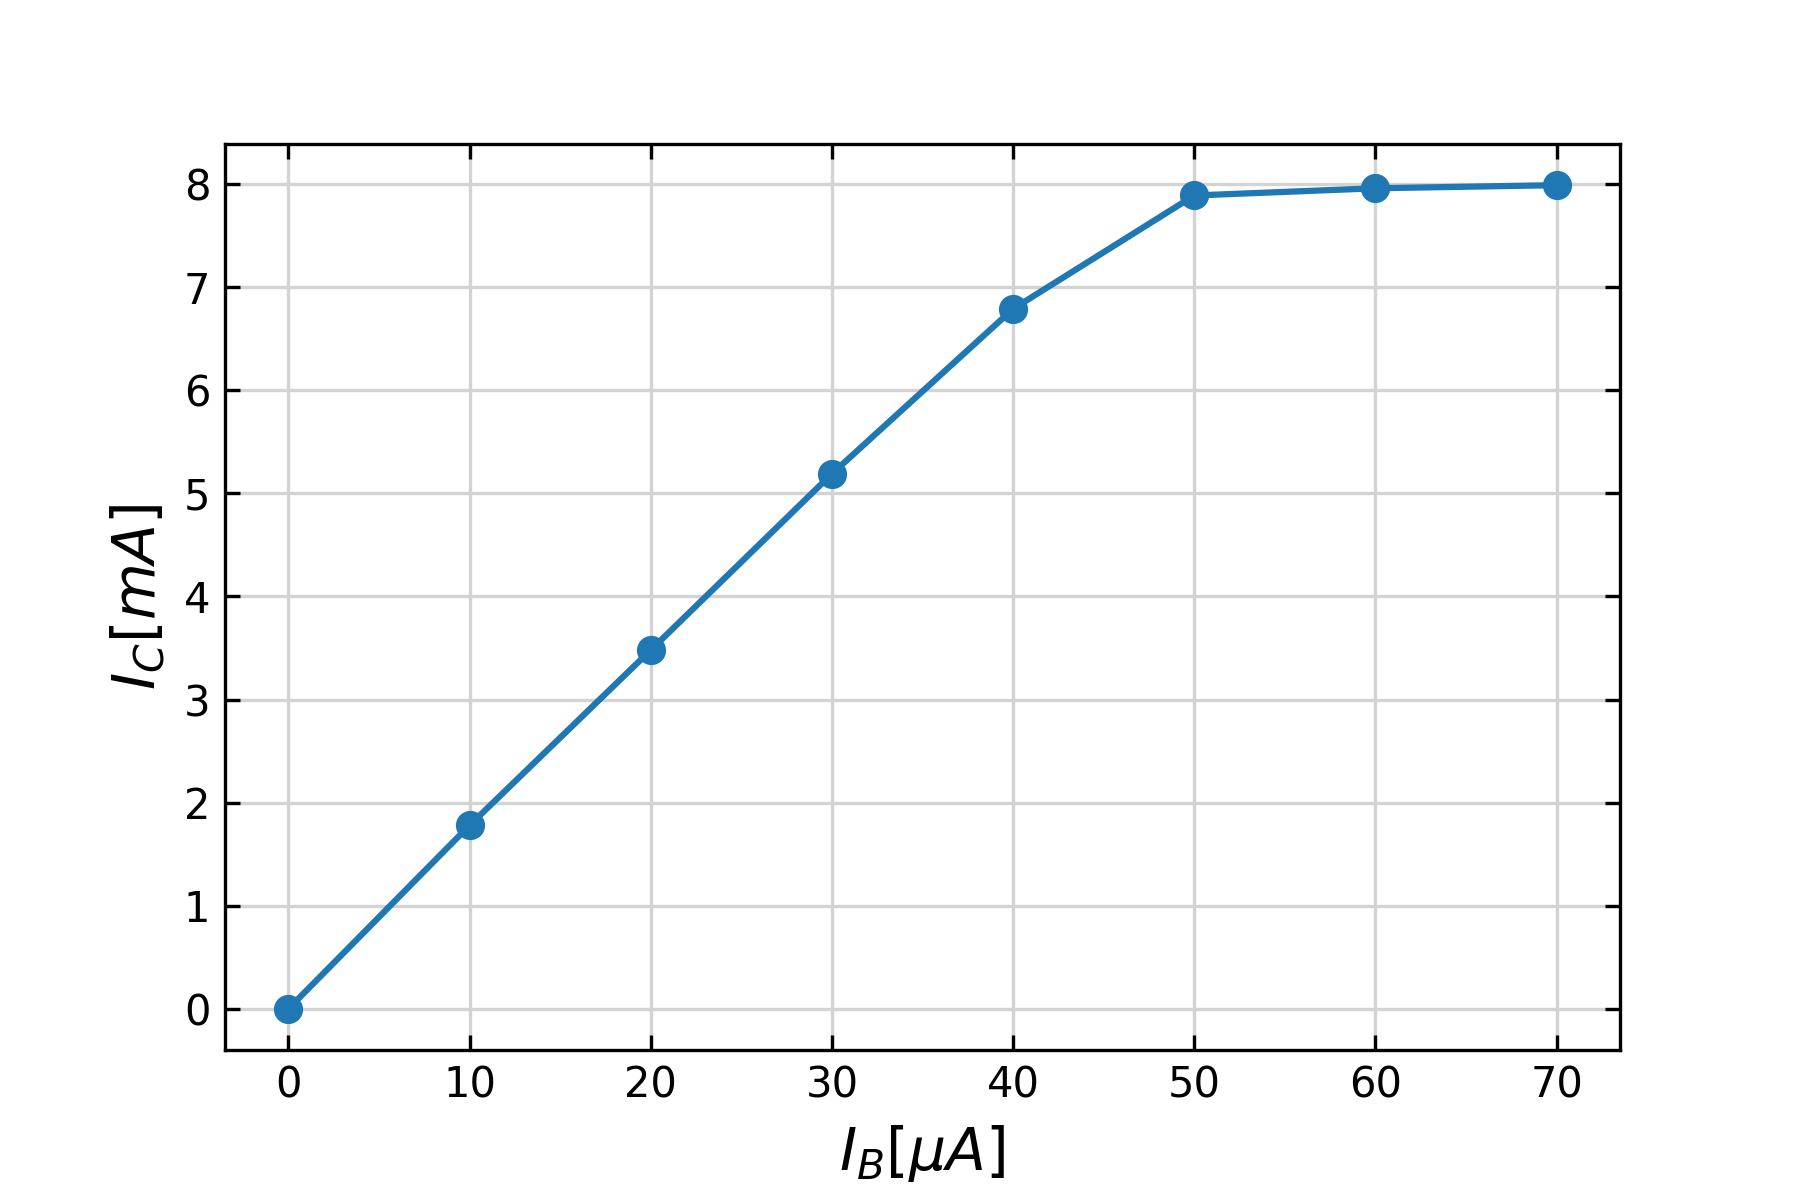
\includegraphics[height=50mm]{ex-7.png}
        \caption{$Tr_1$の電流増幅特性}
        \label{ex:7}
    \end{figure}

    以下,表\ref{tbl:8}に$Tr_2$の測定結果の表を,図\ref{ex:8}の測定結果のグラフを示す.
    \begin{table}[H]
        \centering
        \caption{$Tr_2$の電流増幅特性の測定値}
        \label{tbl:8}
        \small
        \begin{tabular}{|l|l|}
        \hline
        $I_B[\mu A]$ & $I_C[mA]$ \\ \hline
        0            & 0         \\ \hline
        10           & 1.7       \\ \hline
        20           & 3.42      \\ \hline
        22           & 3.75      \\ \hline
        23           & 3.95      \\ \hline
        24           & 4.1       \\ \hline
        25           & 4.3       \\ \hline
        30           & 5.13      \\ \hline
        40           & 6.7       \\ \hline
        50           & 7.9       \\ \hline
        60           & 7.95      \\ \hline
        70           & 7.99      \\ \hline
        \end{tabular}
        \normalsize
    \end{table}
    \begin{figure}[H]
        \centering
        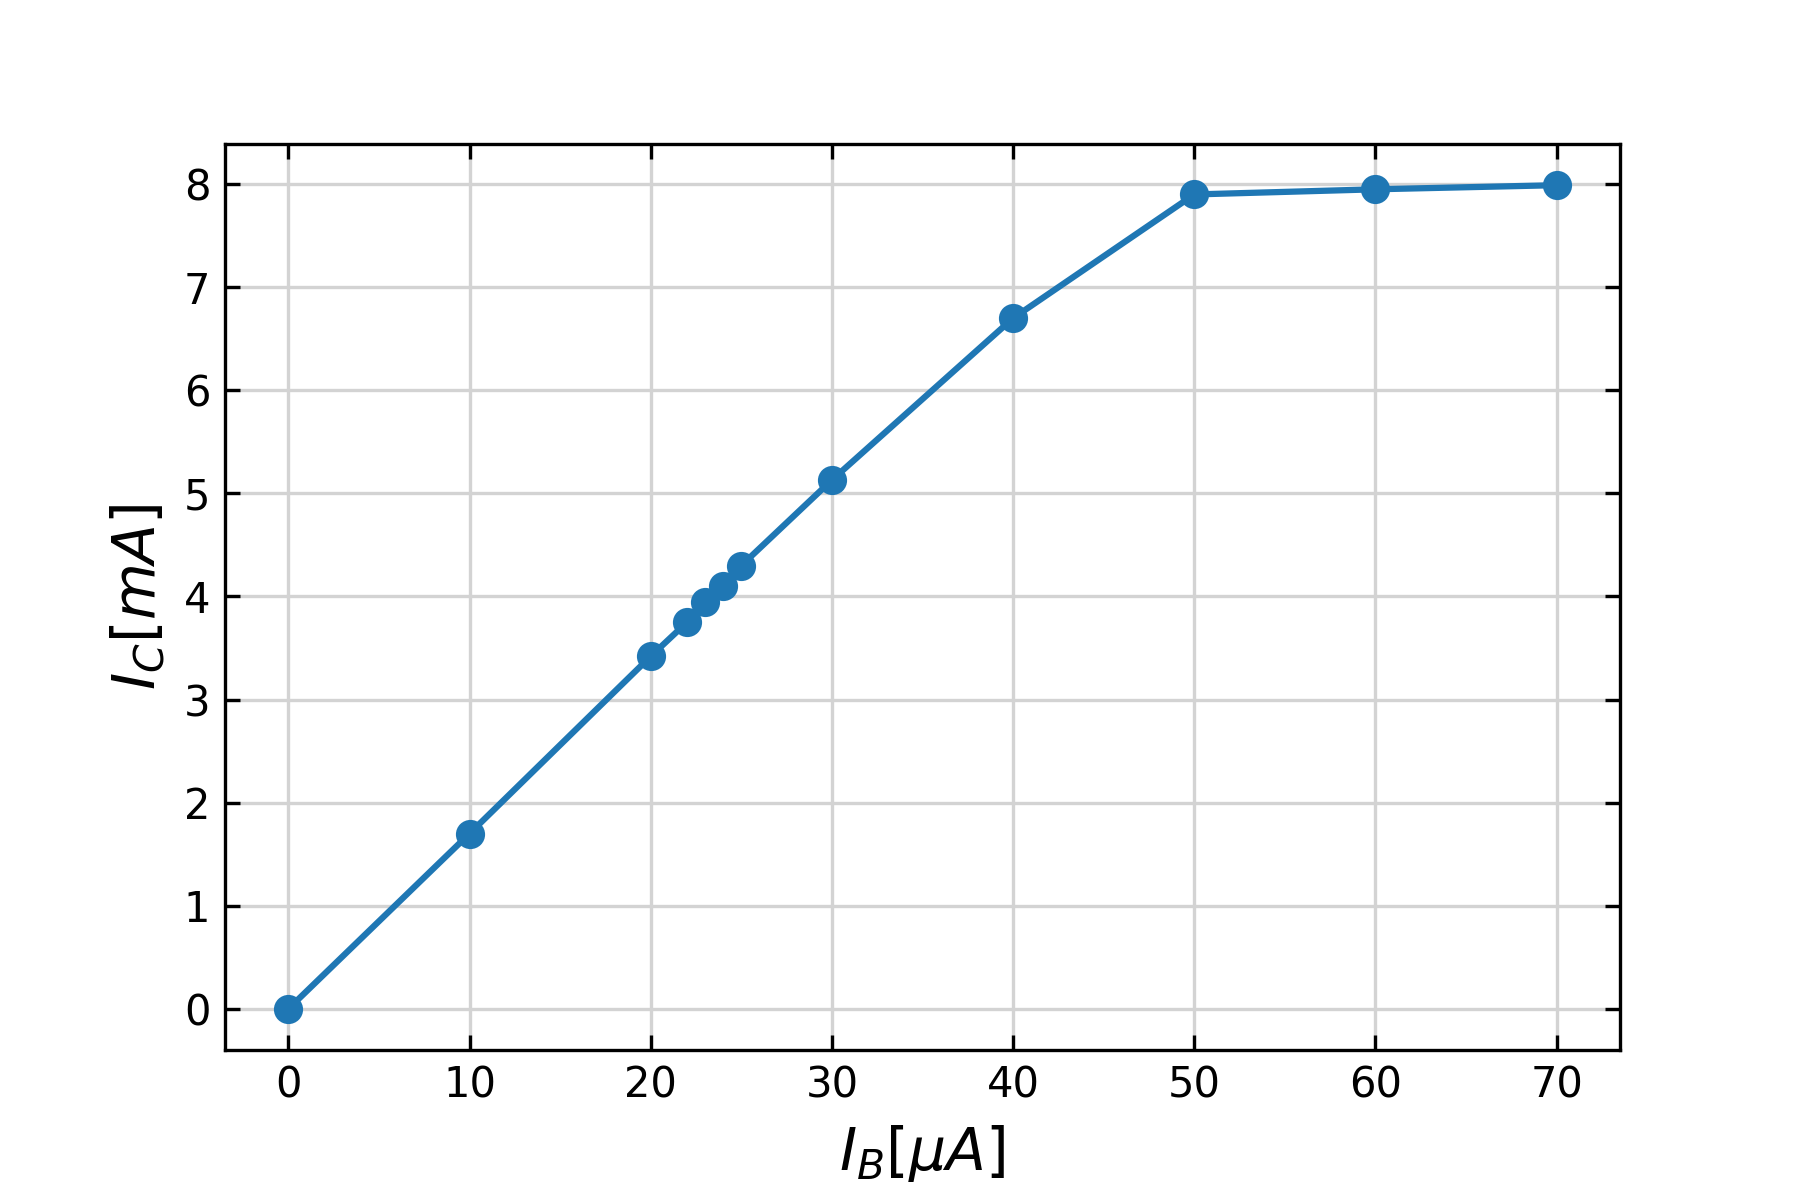
\includegraphics[height=50mm]{ex-8.png}
        \caption{$Tr_2$の電流増幅特性}
        \label{ex:8}
    \end{figure}

    以下,表\ref{tbl:9}に$Tr_3$の測定結果の表を,図\ref{ex:9}の測定結果のグラフを示す.
    \begin{table}[H]
        \centering
        \caption{$Tr_3$の電流増幅特性の測定値}
        \label{tbl:9}
        \small
        \begin{tabular}{|l|l|}
        \hline
        $I_B[\mu A]$ & $I_C[mA]$ \\ \hline
        0            & 0         \\ \hline
        10           & 1.8       \\ \hline
        20           & 3.56      \\ \hline
        30           & 5.28      \\ \hline
        40           & 7.93      \\ \hline
        50           & 7.94      \\ \hline
        60           & 7.98      \\ \hline
        70           & 7.99      \\ \hline
        \end{tabular}
        \normalsize
    \end{table}
    \begin{figure}[H]
        \centering
        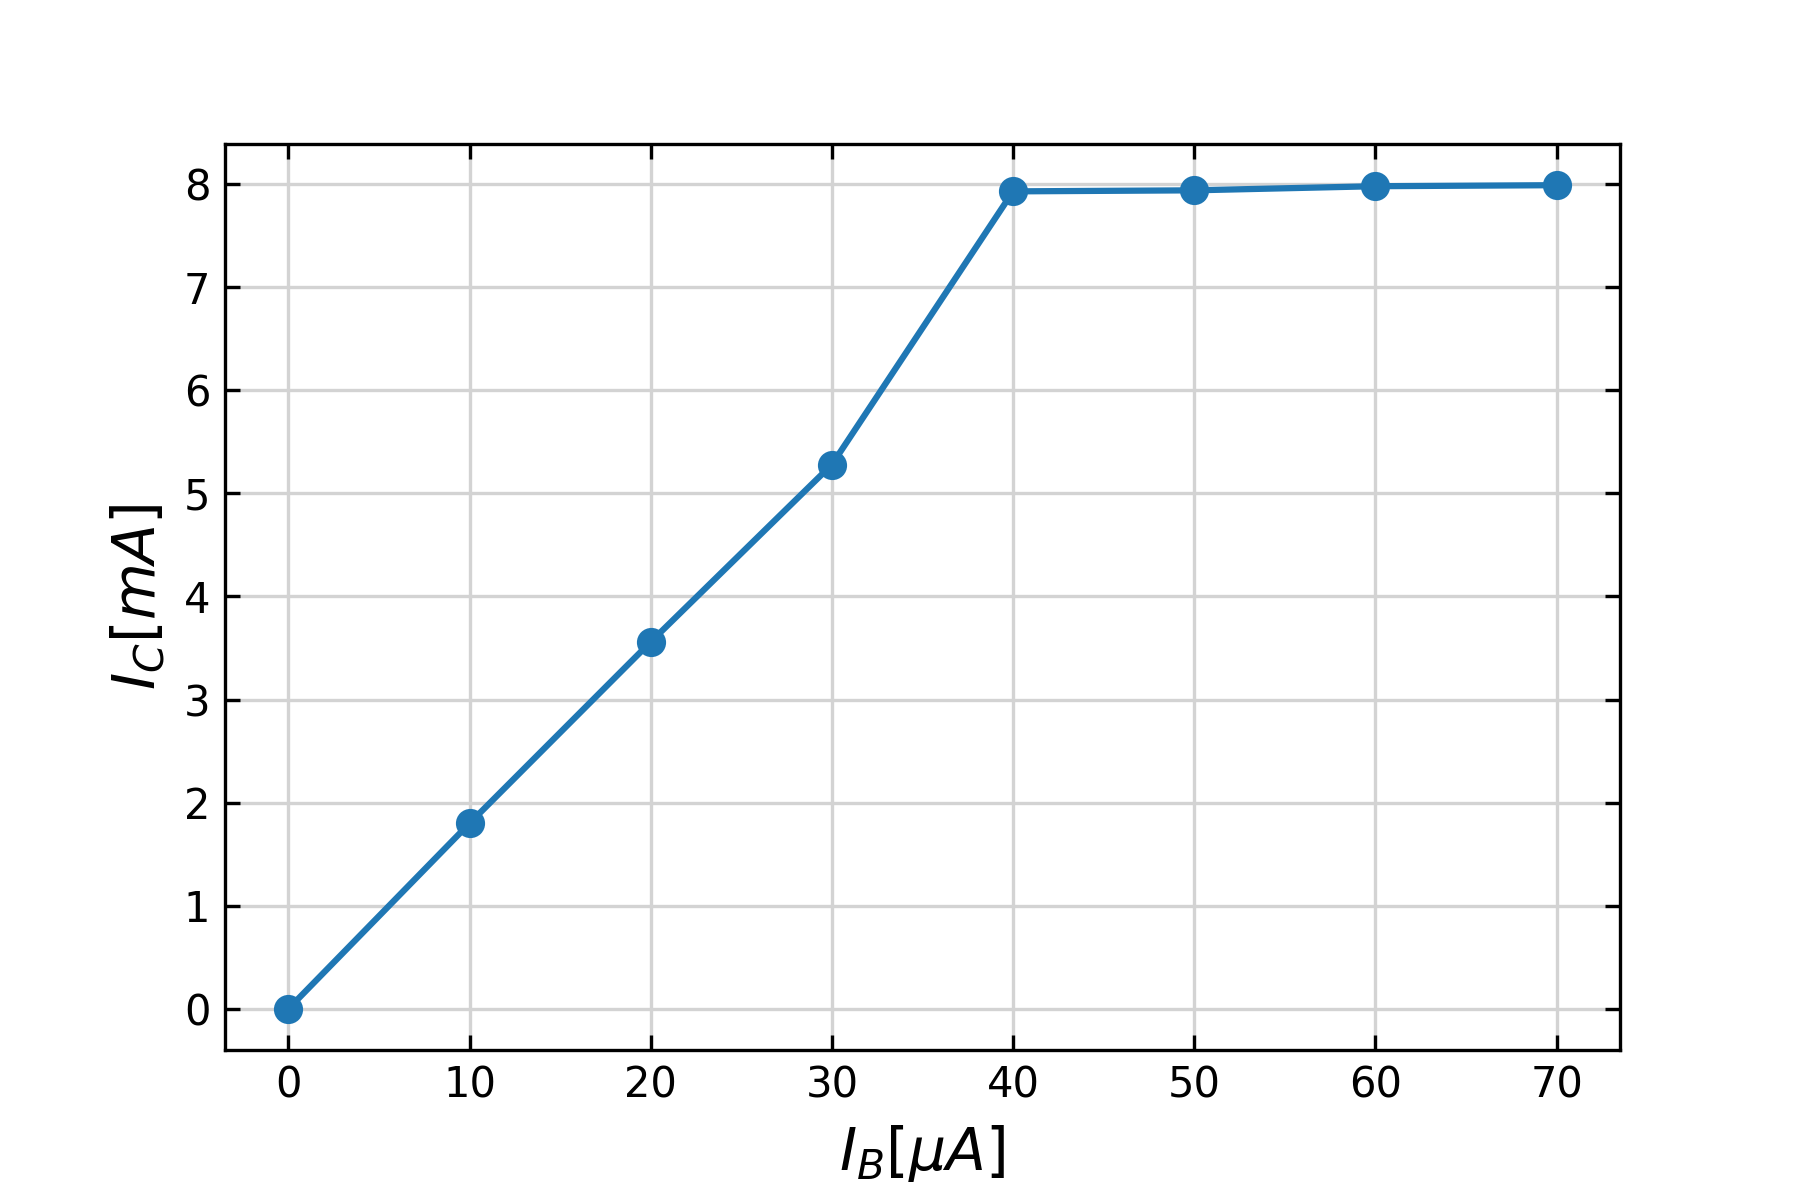
\includegraphics[height=50mm]{ex-9.png}
        \caption{$Tr_3$の電流増幅特性}
        \label{ex:9}
    \end{figure}

    \newpage
    \subsubsection{電圧増幅特性の測定方法}
    1.2.2に示した測定を,$Tr_2$について行った.\\
    以後,トランジスタは$Tr_2$を使用した.\\
    以下,表\ref{tbl:10}に測定結果の表を,図\ref{ex:10}の測定結果のグラフを示す.
    \begin{table}[H]
        \centering
        \caption{電圧増幅特性の測定値}
        \label{tbl:10}
        \small
        \begin{tabular}{|l|l|}
        \hline
        $V_{BE}[V]$ & $V_{CE}[V]$ \\ \hline
        0.1         & 8.02        \\ \hline
        0.2         & 8.02        \\ \hline
        0.3         & 8.02        \\ \hline
        0.4         & 8.02        \\ \hline
        0.5         & 8.02        \\ \hline
        0.559       & 7.97        \\ \hline
        0.61        & 7.71        \\ \hline
        0.629       & 7.4         \\ \hline
        0.641       & 7.08        \\ \hline
        0.653       & 6.59        \\ \hline
        0.668       & 5.6         \\ \hline
        0.675       & 4.93        \\ \hline
        0.685       & 3.77        \\ \hline
        0.701       & 1.85        \\ \hline
        0.712       & 0.645       \\ \hline
        0.713       & 0.245       \\ \hline
        0.715       & 0.159       \\ \hline
        0.717       & 0.127       \\ \hline
        \end{tabular}
        \normalsize
    \end{table}
    \begin{figure}[H]
        \centering
        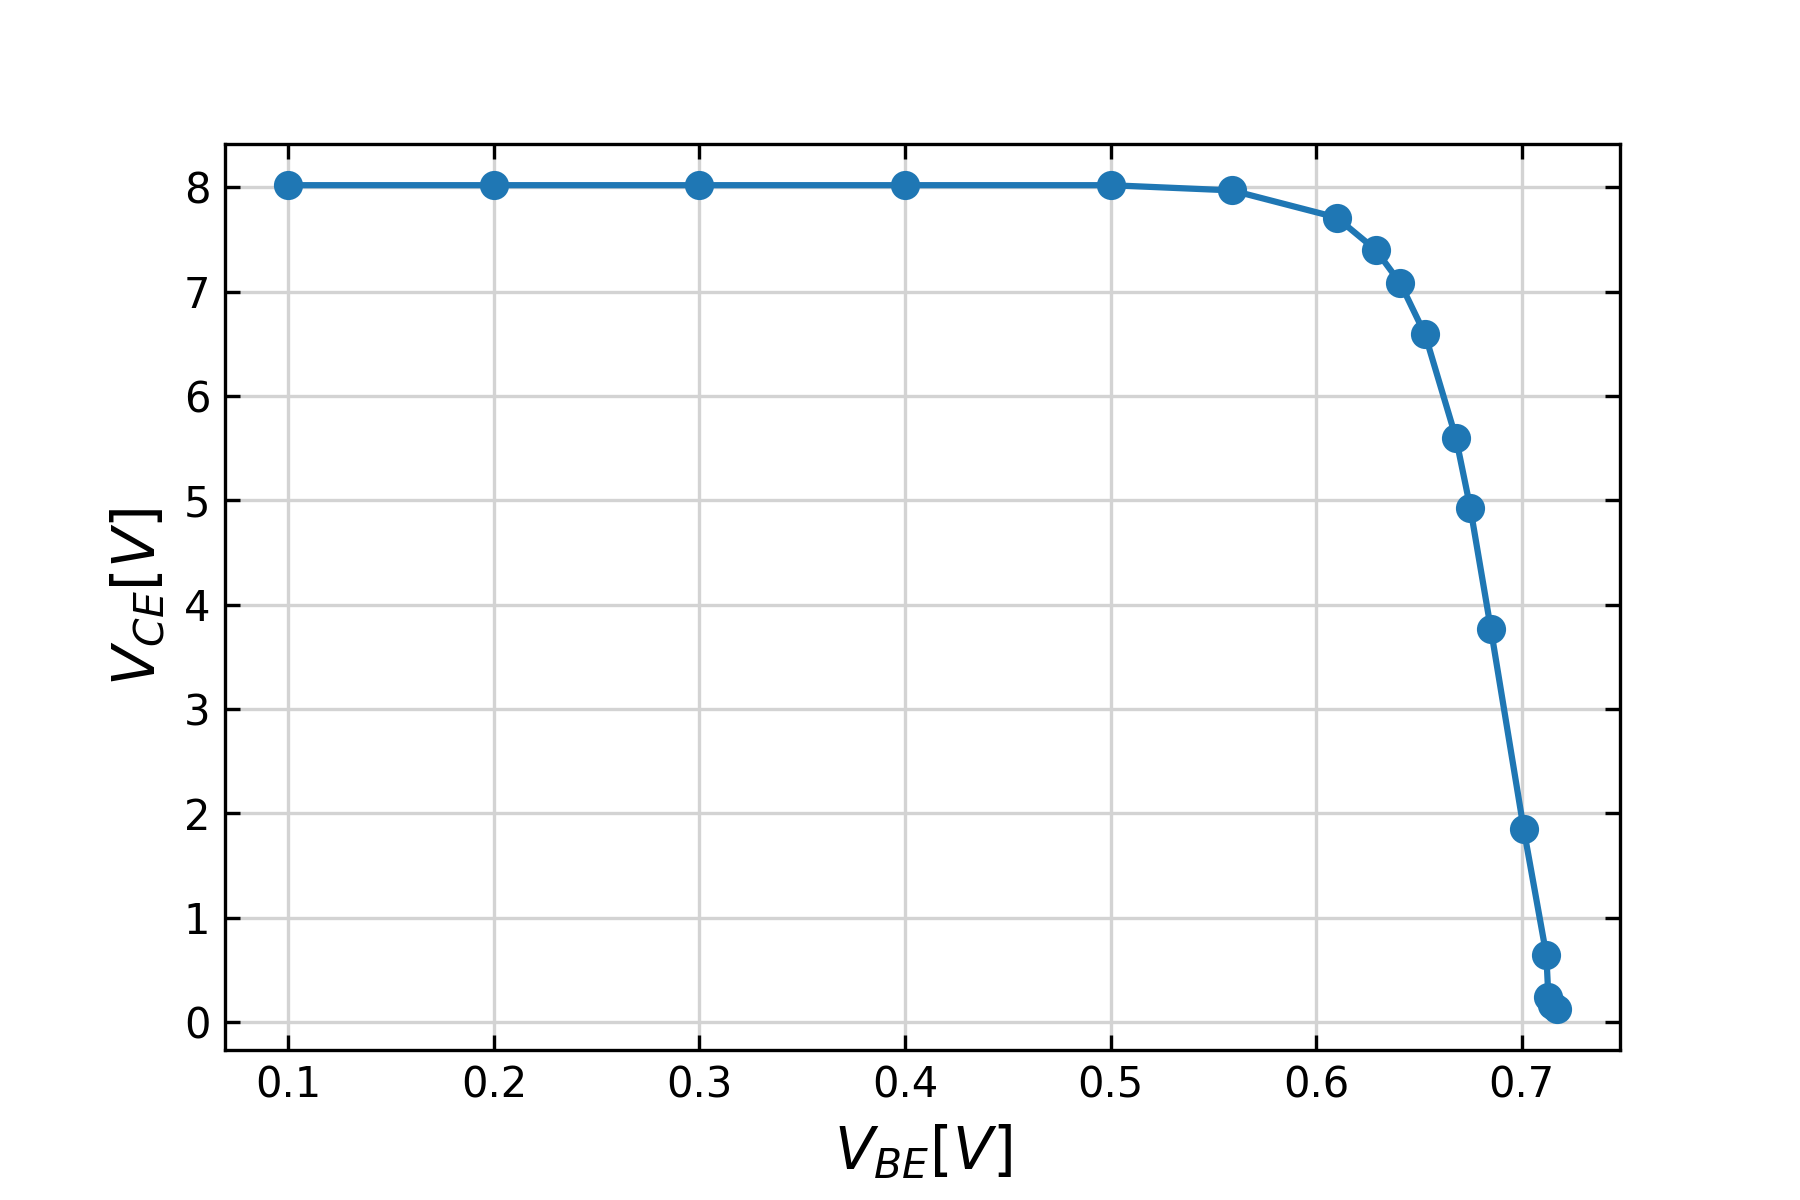
\includegraphics[height=50mm]{ex-10.png}
        \caption{電圧増幅特性}
        \label{ex:10}
    \end{figure}

    \subsubsection{直流バイアス回路定数の選定およびバイアス電圧測定}
    \begin{wrapfigure}{r}{70mm}
        \vspace*{-\intextsep}
        \begin{center}
            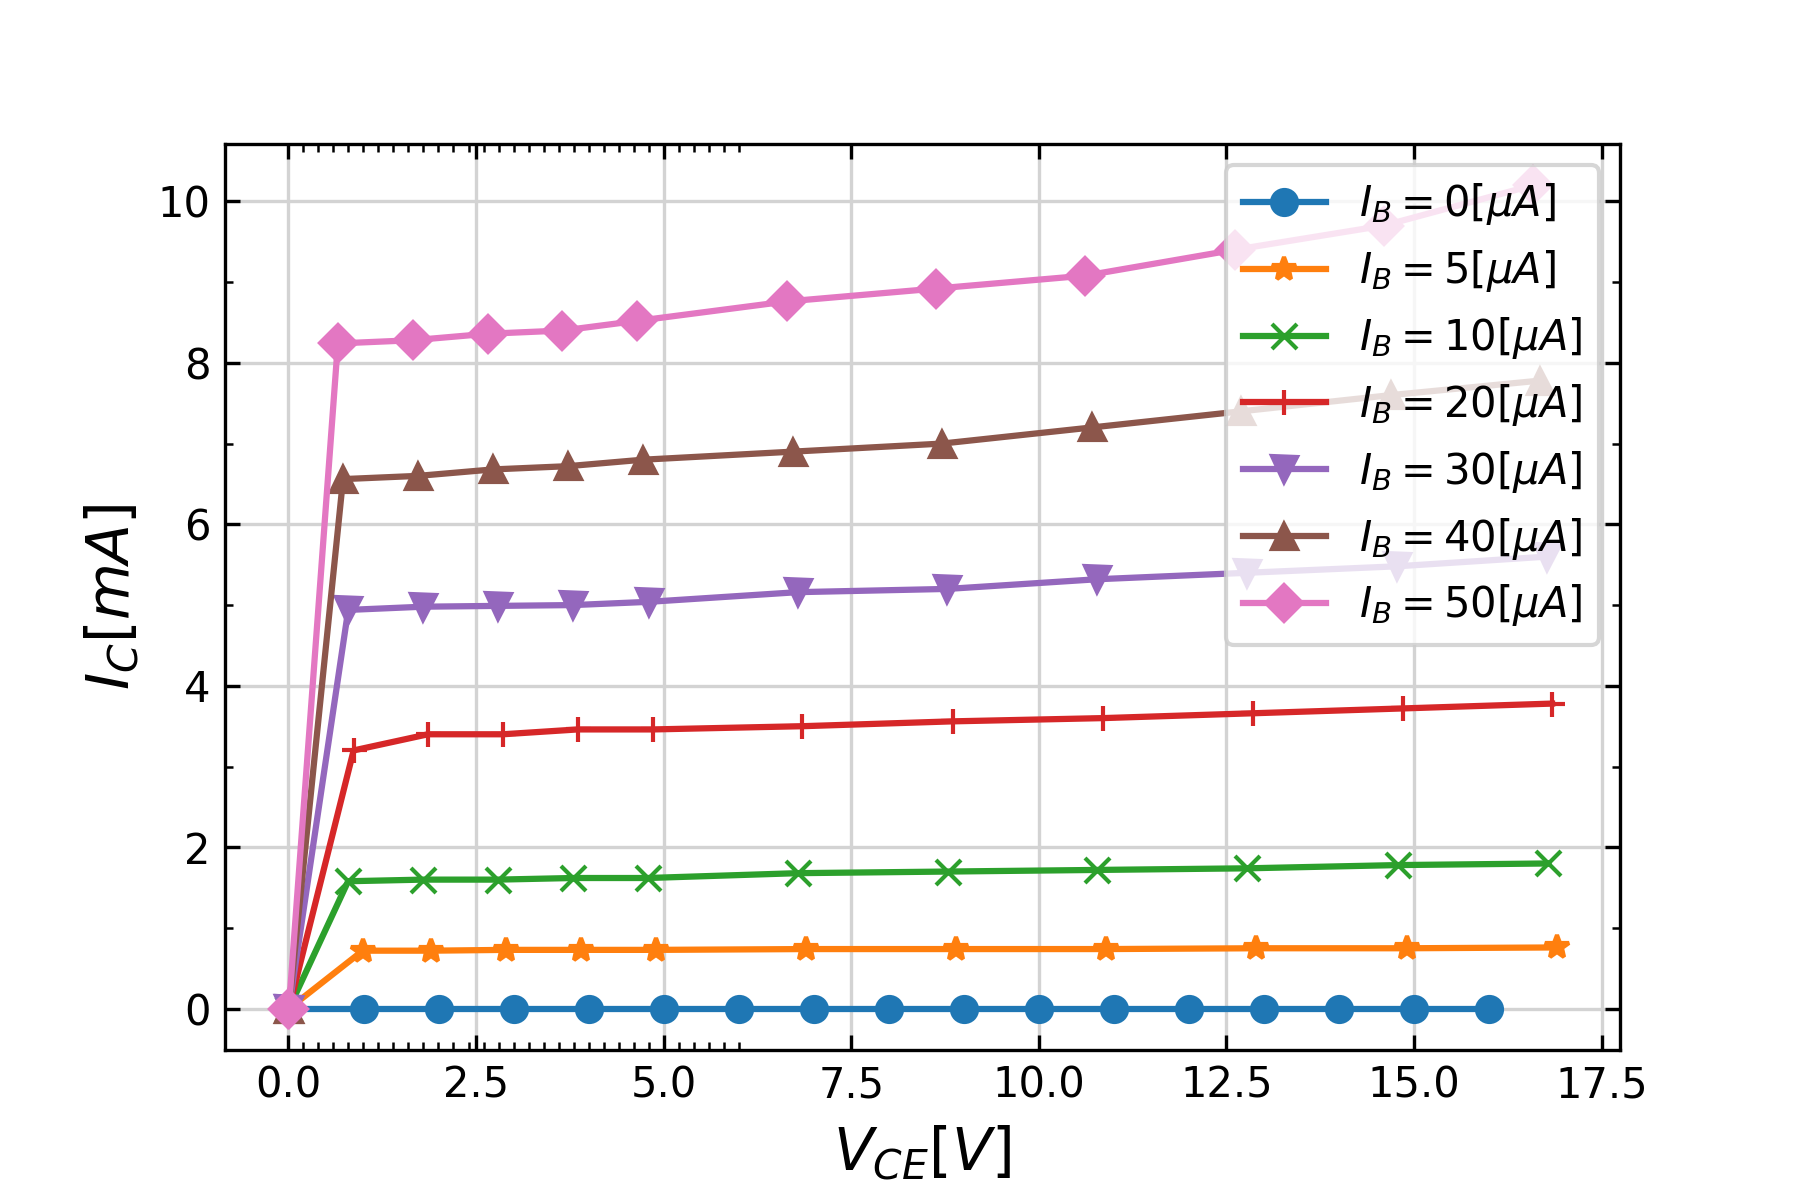
\includegraphics[height=50mm]{ex-5.png}
            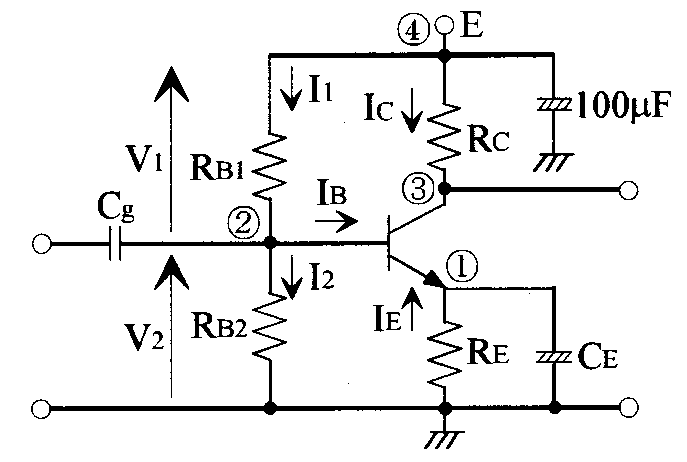
\includegraphics[height=40mm]{fig-10.png}
            \caption{出力特性測定回路}
        \end{center}
    \end{wrapfigure}
    先の実験で測定した出力特性に$8[V]$,$R_C$の交流負荷線を引き,動作点を記入する.\\ 
    \begin{equation}
        E_C = R_C I_C + V_{CE}
    \end{equation}
    また,動作点を通る傾き$1/(R_C + R_E)$の直流負荷線を引き,電源電圧を決定する.\\
    ここでは$R_C = R_E = 1k\Omega$とする.

    以下の下線部を埋めて実験を行う.\\
    Trの名称 \underline{VTC C1815 L VDH ($Tr_2$)}\\
    交流負荷線 $R_C = $    \underline{1000}$\Omega$\\
    直流負荷線 $R_C + R_E = $  \underline{2000}$\Omega$\\
               $R_E = $     \underline{1000}$\Omega$\\
    \\
    電源電圧 $E = $ \underline{12}$V$\\
    設定した動作点Qにおける\\
    ベース電流 $I_{BQ} = $ \underline{23}$\mu A$\\
    コレクタ電流 $I_{CQ} = $ \underline{3.95}$mA$\\
    電流増幅率 \underline{171.7}\\
    ベース-エミッタ間電圧 $V_{BEQ} = $ \underline{0.674}$V$\\
    コレクタ-エミッタ間電圧 $V_{CEQ} = $ \underline{4}$V$\\
    \\
    静特性から,図\ref{fig:10}における各点の電位は,\\
    \hspace{7mm}\textcircled{\scriptsize 1} \underline{4}$V$\hspace{7mm}\textcircled{\scriptsize 2} \underline{4.674}$V$\hspace{7mm}\textcircled{\scriptsize 3} \underline{8}$V$ と求まる.\\
    また,$I_2 = V_2 / R_{B2}$,$I_1 = (E - V_2)$,$I_1 = I_2 + I_{BQ}$の関係が成り立つ.\\
    $I_{BQ}$,$V_1$,$V_2$,$E$は既知である.また,係数$k$を導入し,$I_2 = k I_{BQ}$と表す.これらを用いて$I_1$,$I_2$,$R_{B1}$,$R_{B2}$を式で表すと\\
    \hspace{7mm}$I_1 = $ \underline{$(1+k)I_{BQ}$}\hspace{7mm}$I_2 = $ \underline{$kI_{BQ}$}\hspace{7mm}$R_{B1} = $ \underline{$V_1/\{(1+k)I_{BQ}\}$} $R_{B2} = $ \underline{$V_2/kI_{BQ}$}\\
    となる.$k$の値を変えていくつかの場合について$R_{B1}$,$R_{B2}$の値を求めよ.一番右端の欄には,実験回路に選んだ値を記せ.
    \begin{table}[H]
        \begin{tabular}{||c||c|c|c|c|c|c||c||}
        \hline\hline
        $k$      & $1$             & $5$             & $10$            & $20$            & $30$            & $50$         & $20$            \\ \hline\hline
        $R_{B1}$ & $159.26k\Omega$ & $53.086k\Omega$ & $28.156k\Omega$ & $15.167k\Omega$ & $10.274k\Omega$ & $6245\Omega$ & $15.167k\Omega$ \\ \hline
        $R_{B2}$ & $203.21k\Omega$ & $40.643k\Omega$ & $20.321k\Omega$ & $10.160k\Omega$ & $6773\Omega$    & $4064\Omega$ & $10.160k\Omega$ \\ \hline\hline
        \end{tabular}
    \end{table}
    \newpage
    増幅しようとする周波数範囲は,\hspace{7mm}\underline{200}$Hz$〜\hspace{7mm}\underline{100k}$Hz$\\
    この下限周波数より,$C_g$,$C_E$を決定すると,$C_g = $\underline{0.8665}$\mu F$\hspace{7mm} \underline{148.779}$\mu F$\\
    各点の電位及び電圧
    \begin{table}[H]
        \begin{tabular}{||c||c|c|c||c||c|c|c||}
        \hline\hline
        点                                                           & 設計値   & 実測値   & 誤差 & 点                                                           & 設計値   & 実測値   & 誤差 \\ \hline\hline
        \textbackslash{}textcircled\{\textbackslash{}scriptsize 1\} & 4     & 3.998 &    & $\textcircled{\scriptsize 3} - \textcircled{\scriptsize 1}$ & 4     & 4.028 &    \\ \hline
        \textbackslash{}textcircled\{\textbackslash{}scriptsize 2\} & 4.674 & 4.668 &    & $\textcircled{\scriptsize 2} - \textcircled{\scriptsize 1}$ & 0.674 & 0.670 &    \\ \hline
        \textbackslash{}textcircled\{\textbackslash{}scriptsize 3\} & 8     & 8.027 &    & $\textcircled{\scriptsize 4} - \textcircled{\scriptsize 2}$ & 7.326 & 7.312 &    \\ \hline
        \textbackslash{}textcircled\{\textbackslash{}scriptsize 4\} & 12    & 11.99 &    & $\textcircled{\scriptsize 4} - \textcircled{\scriptsize 3}$ & 4     & 3.958 &    \\ \hline\hline
        \end{tabular}
    \end{table}

    \subsubsection{入出力特性の測定結果}
    1.2.5に示した測定を,$Tr_2$について行った.\\
    以下,表\ref{tbl:11}に測定結果の表を,図\ref{ex:11}の測定結果のグラフを示す.
    また,図\ref{ex:12}〜\ref{ex:15}にディジタルオシロスコープを用いて測定した入力波形と出力波形を示す.
    \begin{table}[H]
        \centering
        \caption{入出力特性の測定値}
        \label{tbl:11}
        \small
        \begin{tabular}{|l|l|}
        \hline
        $V_i[V]$ & $V_o[V]$ \\ \hline
        0        & 0        \\ \hline
        0.011    & 1.2      \\ \hline
        0.02     & 2        \\ \hline
        0.03     & 2.8      \\ \hline
        0.04     & 3.22     \\ \hline
        0.05     & 3.5      \\ \hline
        0.06     & 3.62     \\ \hline
        0.07     & 3.78     \\ \hline
        0.08     & 3.82     \\ \hline
        0.09     & 3.92     \\ \hline
        0.101    & 3.98     \\ \hline
        0.11     & 4        \\ \hline
        0.121    & 4.02     \\ \hline
        0.13     & 4.04     \\ \hline
        0.14     & 4.06     \\ \hline
        0.15     & 4.1      \\ \hline
        0.16     & 4.1      \\ \hline
        0.171    & 4.14     \\ \hline
        0.18     & 4.14     \\ \hline
        0.19     & 4.16     \\ \hline
        0.203    & 4.18     \\ \hline
        \end{tabular}
        \normalsize
    \end{table}
    \begin{figure}[H]
        \centering
        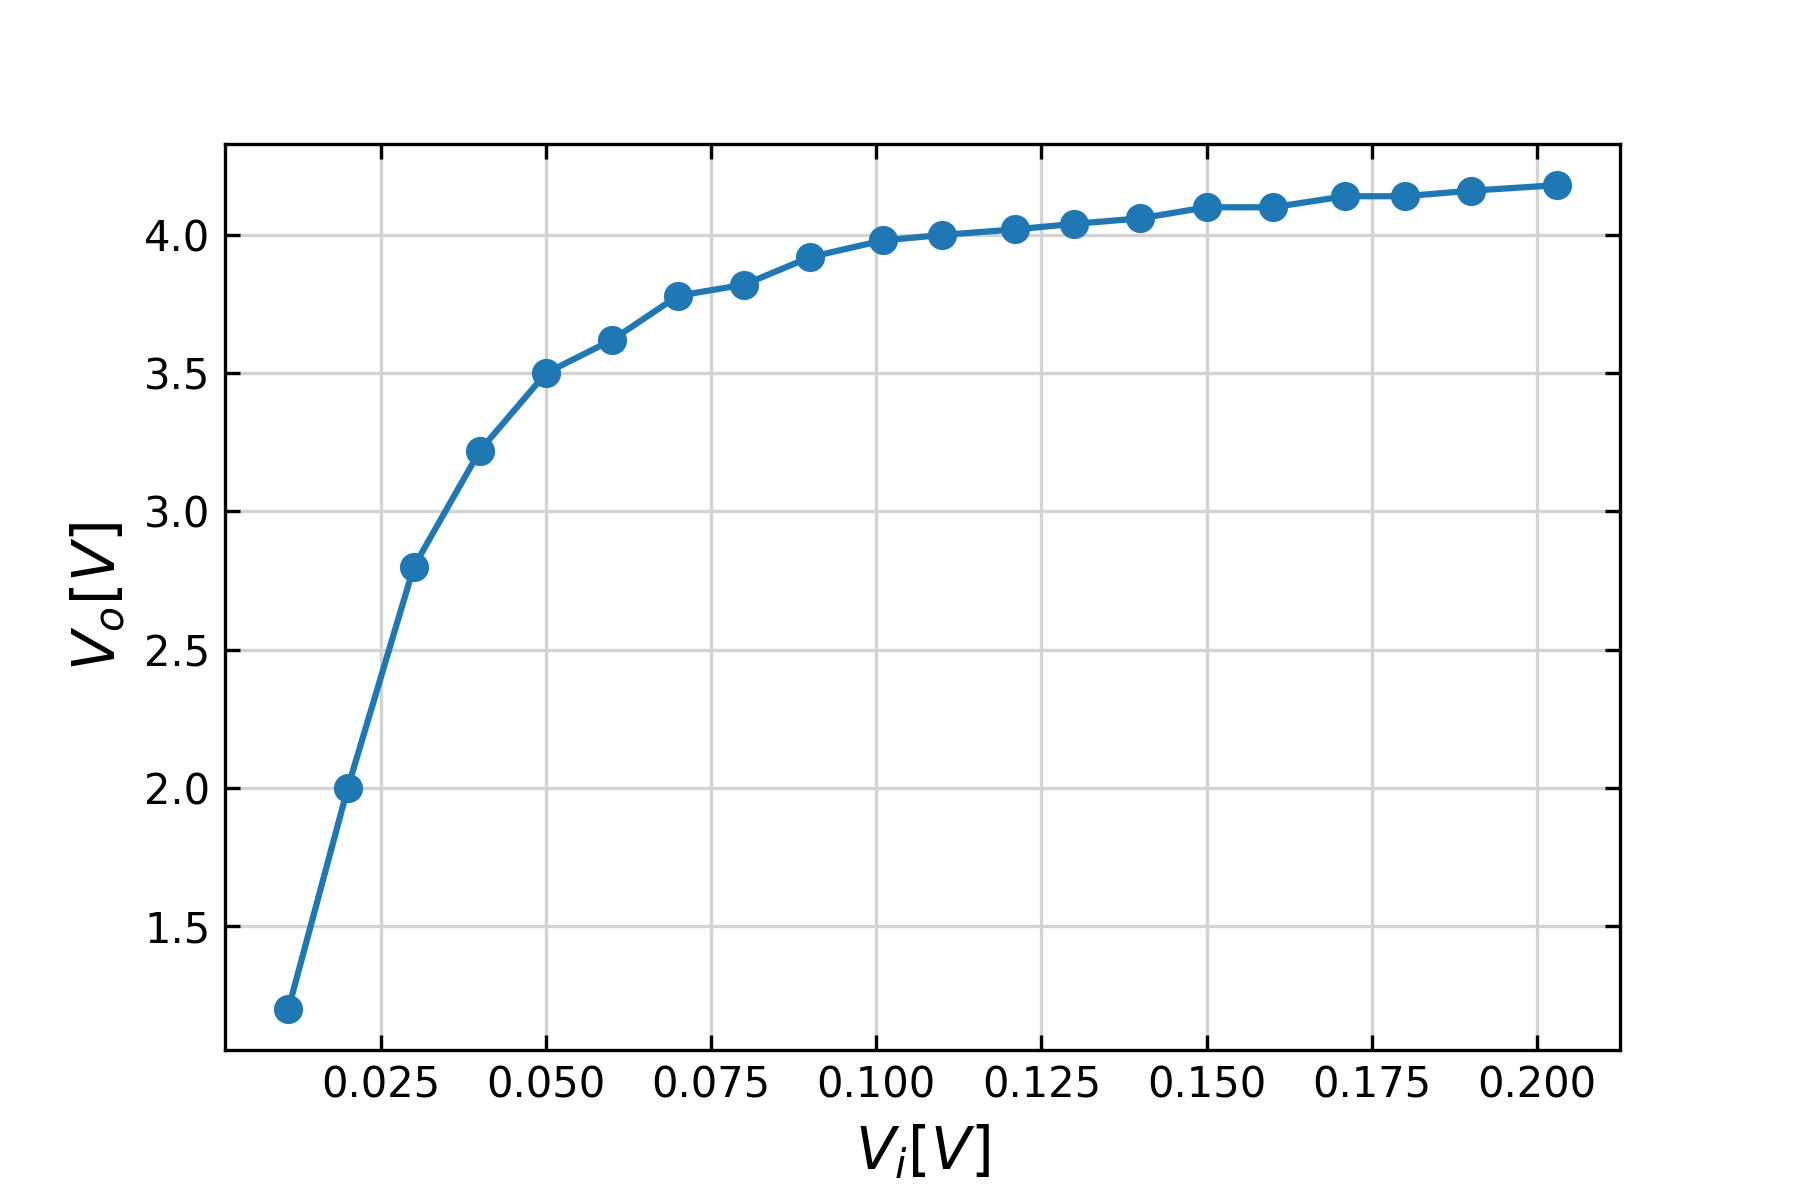
\includegraphics[height=50mm]{ex-11.png}
        \caption{入出力特性}
        \label{ex:11}
    \end{figure}
    \begin{figure}[H]
        \centering
        \includegraphics[height=80mm]{ex-12.bmp}
        \caption{入力電圧 $0.011[V]$のときの波形}
        \label{ex:12}
    \end{figure}
    \begin{figure}[H]
        \centering
        \includegraphics[height=80mm]{ex-13.bmp}
        \caption{入力電圧 $0.04[V]$のときの波形}
        \label{ex:13}
    \end{figure}
    \begin{figure}[H]
        \centering
        \includegraphics[height=80mm]{ex-14.bmp}
        \caption{入力電圧 $0.101[V]$のときの波形}
        \label{ex:14}
    \end{figure}
    \begin{figure}[H]
        \centering
        \includegraphics[height=80mm]{ex-15.bmp}
        \caption{入力電圧 $0.203[V]$のときの波形}
        \label{ex:15}
    \end{figure}

    \newpage
    \subsubsection{周波数特性の測定}
    1.2.6に示した測定を,$Tr_2$について行った.
    以下,表\ref{tbl:12}〜\ref{tbl:14}に測定結果の表を,図\ref{ex:16}の測定結果のグラフを示す.
    \begin{table}[H]
        \centering
        \caption{周波数特性の測定値 ($C_E = 100[\mu F]$)}
        \label{tbl:12}
        \small
        \begin{tabular}{|l|l|l|l|}
        \hline
        $V_i[V]$ & $V_o[V]$ & $frequency[Hz]$ & $Amplification degree[dB]$ \\ \hline
        0.01     & 0.0276   & 10              & 8.81818164130435           \\ \hline
        0.01     & 0.0828   & 20              & 18.3606067356976           \\ \hline
        0.01     & 0.138    & 30              & 22.7975817280247           \\ \hline
        0.01     & 0.192    & 40              & 25.666024574071            \\ \hline
        0.01     & 0.242    & 50              & 27.6763073196086           \\ \hline
        0.01     & 0.292    & 60              & 29.3076570289684           \\ \hline
        0.01     & 0.34     & 70              & 30.6295783408451           \\ \hline
        0.01     & 0.385    & 80              & 31.70921459017             \\ \hline
        0.01     & 0.424    & 90              & 32.5473171318547           \\ \hline
        0.01     & 0.472    & 100             & 33.4788399726818           \\ \hline
        0.01     & 0.78     & 200             & 37.8418920538096           \\ \hline
        0.01     & 0.95     & 300             & 39.554472105777            \\ \hline
        0.01     & 1.04     & 400             & 40.3406667859756           \\ \hline
        0.01     & 1.09     & 500             & 40.7485299588125           \\ \hline
        0.01     & 1.14     & 750             & 41.1380970267295           \\ \hline
        0.01     & 1.17     & 1000            & 41.3637172349232           \\ \hline
        0.01     & 1.2      & 2000            & 41.5836249209525           \\ \hline
        0.01     & 1.2      & 3000            & 41.5836249209525           \\ \hline
        0.01     & 1.2      & 5000            & 41.5836249209525           \\ \hline
        0.01     & 1.2      & 7500            & 41.5836249209525           \\ \hline
        0.01     & 1.2      & 10000           & 41.5836249209525           \\ \hline
        0.01     & 1.2      & 25000           & 41.5836249209525           \\ \hline
        0.01     & 1.2      & 50000           & 41.5836249209525           \\ \hline
        0.01     & 1.2      & 75000           & 41.5836249209525           \\ \hline
        0.01     & 1.18     & 100000          & 41.4376401461225           \\ \hline
        0.01     & 1.1      & 200000          & 40.8278537031645           \\ \hline
        0.01     & 0.98     & 300000          & 39.8245215138499           \\ \hline
        0.01     & 0.85     & 400000          & 38.5883785142859           \\ \hline
        0.01     & 0.75     & 500000          & 37.501225267834            \\ \hline
        0.01     & 0.65     & 600000          & 36.2582671328571           \\ \hline
        0.01     & 0.57     & 700000          & 35.1174971134498           \\ \hline
        0.01     & 0.5      & 800000          & 33.9794000867204           \\ \hline
        0.01     & 0.44     & 900000          & 32.8690535297237           \\ \hline
        0.01     & 0.4      & 1000000         & 32.0411998265592           \\ \hline
        \end{tabular}
        \normalsize
    \end{table}
    \begin{table}[H]
        \centering
        \caption{周波数特性の測定値 ($C_E = 220[\mu F]$)}
        \label{tbl:13}
        \small
        \begin{tabular}{|l|l|l|l|}
        \hline
        $V_i[V]$ & $V_o[V]$ & $frequency[Hz]$ & $Amplification degree[dB]$ \\ \hline
        0.01     & 0.055    & 10              & 14.8072537898849           \\ \hline
        0.01     & 0.175    & 25              & 24.8607609737259           \\ \hline
        0.01     & 0.358    & 50              & 31.0776605328775           \\ \hline
        0.01     & 0.51     & 75              & 34.1514035219587           \\ \hline
        0.01     & 0.63     & 100             & 35.9868109890716           \\ \hline
        0.01     & 1.01     & 250             & 40.0864274756529           \\ \hline
        0.01     & 1.15     & 500             & 41.2139568070722           \\ \hline
        0.01     & 1.18     & 750             & 41.4376401461225           \\ \hline
        0.01     & 1.19     & 1000            & 41.5109392278506           \\ \hline
        0.01     & 1.21     & 2500            & 41.655707406329            \\ \hline
        0.01     & 1.21     & 5000            & 41.655707406329            \\ \hline
        0.01     & 1.21     & 7500            & 41.655707406329            \\ \hline
        0.01     & 1.21     & 10000           & 41.655707406329            \\ \hline
        0.01     & 1.21     & 25000           & 41.655707406329            \\ \hline
        0.01     & 1.21     & 50000           & 41.655707406329            \\ \hline
        0.01     & 1.21     & 75000           & 41.655707406329            \\ \hline
        0.01     & 1.2      & 100000          & 41.5836249209525           \\ \hline
        0.01     & 1.05     & 250000          & 40.4237859813988           \\ \hline
        0.01     & 0.75     & 500000          & 37.501225267834            \\ \hline
        0.01     & 0.54     & 750000          & 34.6478751964594           \\ \hline
        0.01     & 0.4      & 1000000         & 32.0411998265592           \\ \hline
        \end{tabular}
        \normalsize
    \end{table}
    \begin{table}[H]
        \centering
        \caption{周波数特性の測定値 ($C_E = 47[\mu F]$)}
        \label{tbl:14}
        \small
        \begin{tabular}{|l|l|l|l|}
        \hline
        $V_i[V]$ & $V_o[V]$ & $frequency[Hz]$ & $Amplification degree[dB]$ \\ \hline
        0.01     & 0.01     & 10              & 0                          \\ \hline
        0.01     & 0.064    & 25              & 16.1235994796777           \\ \hline
        0.01     & 0.148    & 50              & 23.4052343078991           \\ \hline
        0.01     & 0.224    & 75              & 27.0049603666833           \\ \hline
        0.01     & 0.298    & 100             & 29.4843252815251           \\ \hline
        0.01     & 0.62     & 250             & 35.8478337899651           \\ \hline
        0.01     & 0.86     & 500             & 38.6899690248714           \\ \hline
        0.01     & 0.95     & 750             & 39.554472105777            \\ \hline
        0.01     & 0.99     & 1000            & 39.912703891951            \\ \hline
        0.01     & 1.4      & 2500            & 42.9225607135648           \\ \hline
        0.01     & 1.4      & 5000            & 42.9225607135648           \\ \hline
        0.01     & 1.4      & 7500            & 42.9225607135648           \\ \hline
        0.01     & 1.4      & 10000           & 42.9225607135648           \\ \hline
        0.01     & 1.4      & 25000           & 42.9225607135648           \\ \hline
        0.01     & 1.4      & 50000           & 42.9225607135648           \\ \hline
        0.01     & 1.4      & 75000           & 42.9225607135648           \\ \hline
        0.01     & 1.4      & 100000          & 42.9225607135648           \\ \hline
        0.01     & 0.94     & 250000          & 39.462557071994            \\ \hline
        0.01     & 0.68     & 500000          & 36.6501782541247           \\ \hline
        0.01     & 0.49     & 750000          & 33.8039216005703           \\ \hline
        0.01     & 0.38     & 1000000         & 31.5956719323362           \\ \hline
        \end{tabular}
        \normalsize
    \end{table}
    \begin{table}[H]
        \centering
        \caption{周波数特性の測定値 ($C_E = 147[\mu F]$)}
        \label{tbl:14}
        \small
        \begin{tabular}{|l|l|l|l|}
        \hline
        $V_i[V]$ & $V_o[V]$ & $frequency[Hz]$ & $Amplification degree[dB]$ \\ \hline
        0.01     & 0.041    & 10              & 12.2556771343947           \\ \hline
        0.01     & 0.142    & 25              & 23.0457668876611           \\ \hline
        0.01     & 0.305    & 50              & 29.6859967869357           \\ \hline
        0.01     & 0.438    & 75              & 32.829482210082            \\ \hline
        0.01     & 0.568    & 100             & 35.0869667142204           \\ \hline
        0.01     & 0.958    & 250             & 39.6273101815709           \\ \hline
        0.01     & 1.12     & 500             & 40.9843604534036           \\ \hline
        0.01     & 1.16     & 750             & 41.2891597845384           \\ \hline
        0.01     & 1.19     & 1000            & 41.5109392278506           \\ \hline
        0.01     & 1.21     & 2500            & 41.655707406329            \\ \hline
        0.01     & 1.21     & 5000            & 41.655707406329            \\ \hline
        0.01     & 1.21     & 7500            & 41.655707406329            \\ \hline
        0.01     & 1.21     & 10000           & 41.655707406329            \\ \hline
        0.01     & 1.21     & 25000           & 41.655707406329            \\ \hline
        0.01     & 1.21     & 50000           & 41.655707406329            \\ \hline
        0.01     & 1.21     & 75000           & 41.655707406329            \\ \hline
        0.01     & 1.19     & 100000          & 41.5109392278506           \\ \hline
        0.01     & 1.04     & 250000          & 40.3406667859756           \\ \hline
        0.01     & 0.75     & 500000          & 37.501225267834            \\ \hline
        0.01     & 0.54     & 750000          & 34.6478751964594           \\ \hline
        0.01     & 0.41     & 1000000         & 32.2556771343947           \\ \hline
        \end{tabular}
        \normalsize
    \end{table}
    \begin{figure}[H]
        \centering
        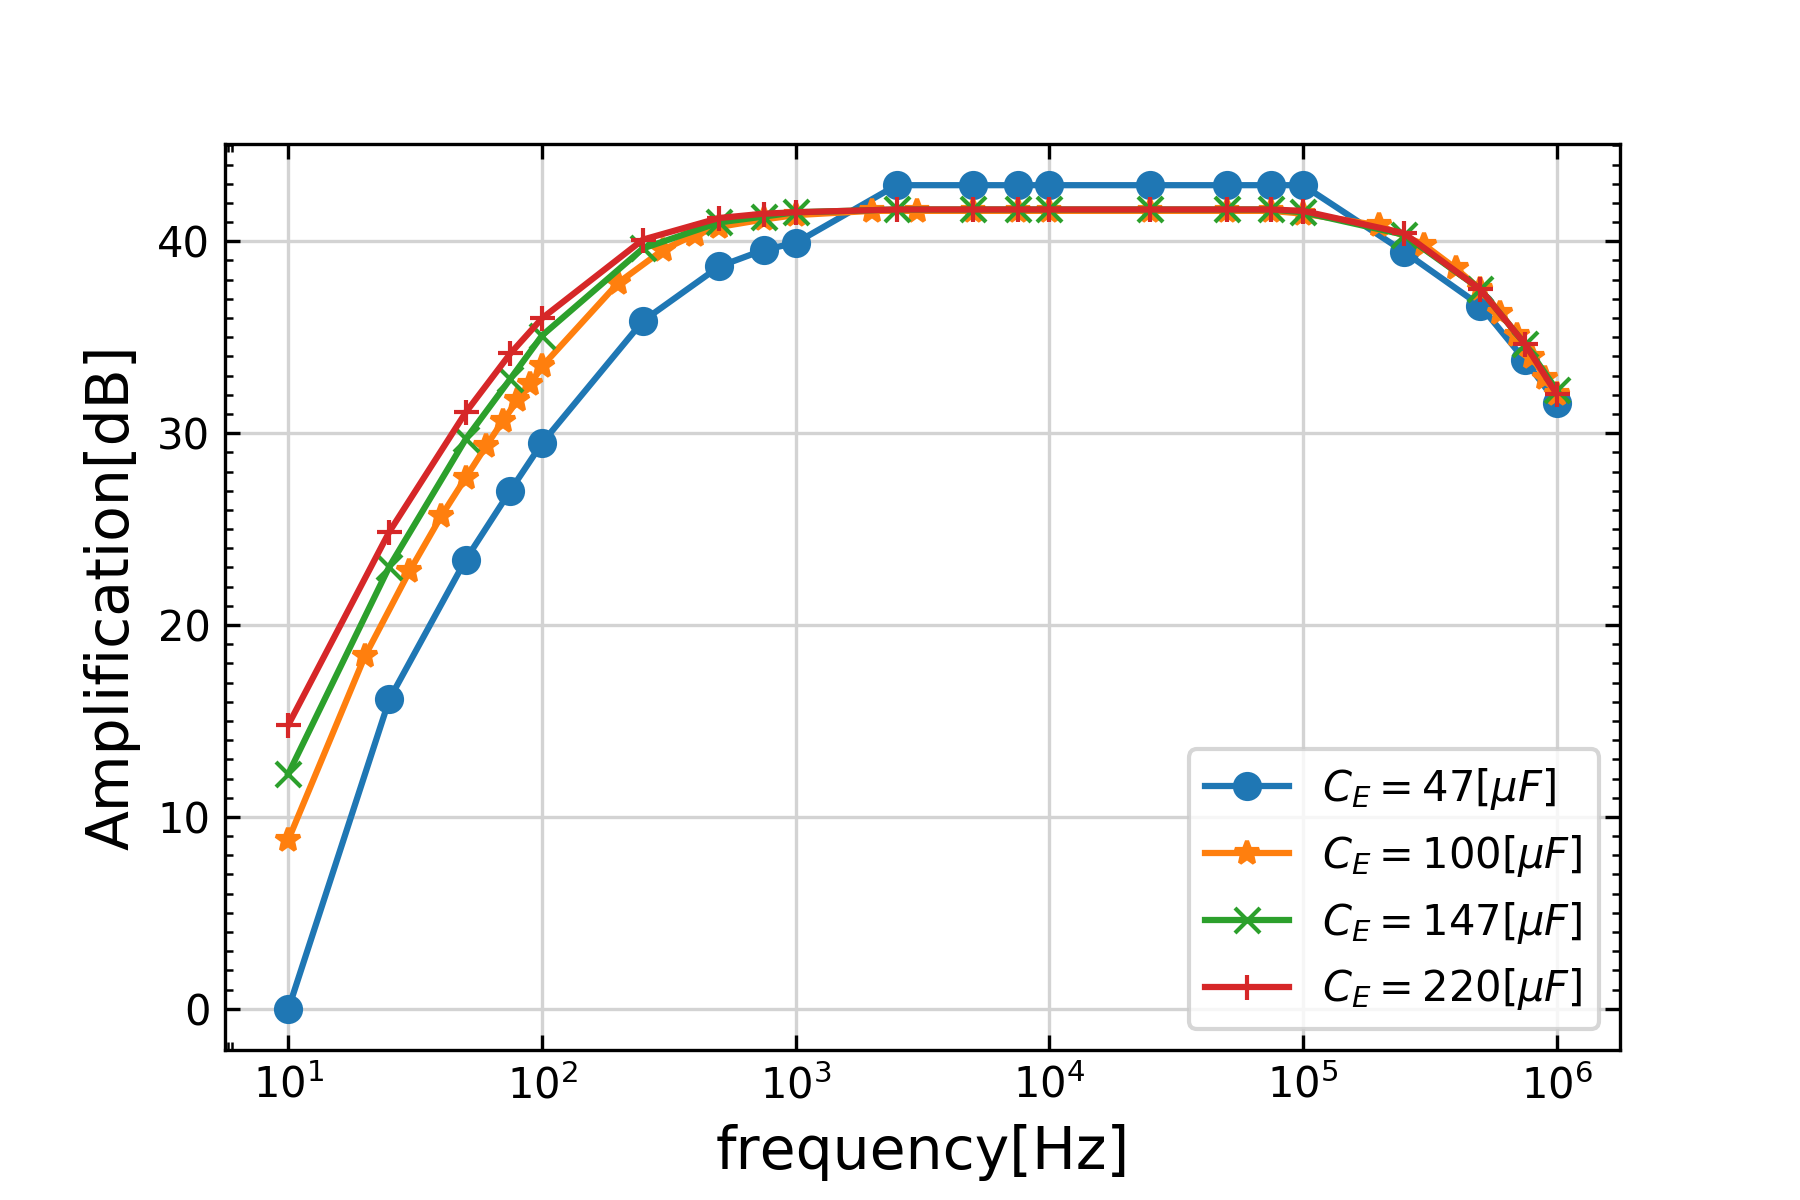
\includegraphics[height=80mm]{ex-16.png}
        \caption{周波数特性}
        \label{ex:16}
    \end{figure}

    % \newpage
    % \section{吟味事項の確認}
    % \subsection{トランジスタの静特性}
    % \subsubsection{1.電圧計,電流計の等級と内部抵抗を調べる.}
    % \subsubsection{2.$V_{CE} = 4[V]$,$I_B = 20[\mu A]$のときの$h$定数を,測定した特性図より求める.}

    % \subsection{トランジスタ増幅}
    


\end{document}